% Je crois que le nouveau guide dit qu'il faut soumettre en 12 points!

\documentclass[12pt,twoside]{memoireuqam1.3}

%\documentclass[11pt,twoside]{memoireuqam1.3}

\usepackage{graphicx}% Pour les figures
\usepackage[french]{babel}

\usepackage[T1]{fontenc}

\usepackage[utf8]{inputenc} % Pour utiliser les caract�res Unicode, notaamment sous Linux
%%%%%%%%%%%%%%%%%%%
% ou
% \usepackage[latin1]{inputenc} % Pour utiliser les accents sous Solaris (?)
% \usepackage[ansinew]{inputenc} % Pour utiliser les caract�res accentu�s sous Windows
% \usepackage[applemac]{inputenc} % Pour utiliser les caract�res accentu�s sous MacOS
%%%%%%%%%%%%%%%%%%%

% Ajouts par Guy T.
% Autres packages souvent utiles
\usepackage{epsfig}
\usepackage{float}
\usepackage{alltt}
\usepackage{graphicx}
\usepackage{url}
%%%%%%%%%%%%%%%%%%%%%%%%%%%%%

% Ajouts par Iulian
% \usepackage{booktabs}	% Pour utiliser ent�te du tableau (commande \midrule)
%%%%%%%%%%%%%%%%%%%%%%%%%%%%%

% Items, and Enum
\newenvironment{Items}%
{\begingroup\setlength{\topsep}{.050\parsep}\addtolength{\parskip}{-.75\parskip}\setlength{\partopsep}{.25\partopsep}%
\begin{itemize}\setlength{\itemsep}{0pt}\addtolength{\parsep}{-.1\parsep}}%
{\end{itemize}\endgroup\smallbreak}

\newenvironment{Enum}%
{\begingroup\setlength{\topsep}{.050\parsep}\addtolength{\parskip}{-.75\parskip}\setlength{\partopsep}{.25\partopsep}%
\begin{enumerate}\setlength{\itemsep}{0pt}\addtolength{\parsep}{-.1\parsep}}%
{\end{enumerate}\endgroup\smallbreak}

\newcommand{\TT}[1]{{\tt #1}}

\newcommand{\ACOMPLETER}{\footnote{??? \`A compl\'eter!!!}}

\newcommand{\AVERIFIER}[1]{\footnote{??? \`A v\'erifier: #1!!!}}

\newtheorem{definition}{D\'efinition}

\floatstyle{boxed}
\newfloat{algorithme}{htbp}{lop}
\floatname{algorithme}{Algorithme}

\floatstyle{ruled}
\newfloat{pseudocode}{htbp}{lop}
\floatname{pseudocode}{Pseudocode}

\newcommand{\ppff}{\texttt{PpFf}}
\newcommand{\PpFf}{\ppff}
  % Pour les d�finitions personnelles

\begin{document}

%%%%%%%%%%%%%%%%%%%%
% Pour la page titre
%%%%%%%%%%%%%%%%%%%%
\title{TRAITEMENT EFFICACE DE FLUX DE DONN\'EES SUR MACHINES MULTI-C\OE{}URS \`A L'AIDE DE FASTFLOW}
\author{Iulian Ciobanu}
\degreemonth{mois du d\'ep\^ot}
\degreeyear{annee du d\'ep\^ot}
\uqammemoire   %% Pour la page titre d'un m�moire
% ou
% \uqamthese   %% Pour la page titre d'une th�se
% ou
% \uqamrapport %% Pour la page titre d'un rapport


\thispagestyle{empty}        % La page titre n'est pas num�rot�e
\maketitle

%%%%%%%%%%%%%%%%%%%%
% Page pr�liminaires
%%%%%%%%%%%%%%%%%%%%
%\renewcommand \bibname{R\'EF\'ERENCES}% FACULTATIF
%Enlever le commentaire, si vous voulez qu'apparaisse le titre R�F�RENCES
% plut�t que BIBLIOGRAPHIE

\renewcommand \listfigurename{LISTE DES FIGURES}
\renewcommand \appendixname{APPENDICE}
\renewcommand \figurename{Figure}
\renewcommand \tablename{Tableau}

\pagenumbering{roman} % num�rotation des pages en chiffres romains
\addtocounter{page}{1} % Pour que les remerciements commencent � la page ii

   \parskip=0pt
   \vspace*{0.1 truecm} 
   \begin{center}
    {\uppercase { REMERCIEMENTS }}\par
   \end{center}
   \nobreak \vspace*{1.10 truecm}
   \parskip=2ex


\GT{Je crois qu'un des évaluateurs n'avait pas aimé <<grand
accomplissement>>.  Il semblait trouver que ça faisait trop
<<pompeux>>~:( À modifier!}

\IC{J'ai remplacé le mot accomplissement par projet.}

\GT{Il est aussi d'usage de remercier le directeur de recherche ou
l'organisme subventionnaire lorsque du support financier a été
offert. J'ai ajouté une phrase à ce  sujet.}

\IC{Oui c'est vrai. Je ne crois pas avoir révié cette section.}

Tout grand projet est rarement r\'ealis\'e par une seule personne. Celui-ci ne fait pas exception. Je suis reconnaissant \`a tous ceux et celles qui m'ont aid\'e et soutenu pendant ces ann\'ees de travail.

Tout d'abord, je voudrais remercier mon directeur de recherche, le professeur Guy Tremblay. Sans son soutien et son aide, ce m\'emoire n'aurait pas pu \^etre termin\'e. Gr\^ace \`a sa riche exp\`erience, il m'a guid\'e dans mes recherches. Il m'a donn\'e de nombreuses id\'ees, suggestions et critiques constructives.
%
Je le remercie aussi pour son support financier au cours de l'hiver et de l'été 2020.

Je dois \'egalement un grand merci au professeur Marco Aldinucci, de l'Universit\'e de Turin, pour son soutien technique pour l'application de \TT{FastFlow}. 

Je souhaite aussi remercier les analystes et techniciens syst\`emes des laboratoires informatiques et le personnel administratif qui ont permis \`a mon m\'emoire de se d\'erouler sans obstacle technique ou administratif.

Enfin, je tiens \`a remercier \`a ma famille, qui a toujours \'et\'e l\`a, m'ayant aid\'e moralement \`a surmonter les difficult\'es que j'ai eues durant ces ann\'ees de recherche. 




\pagenumbering{arabic}
\tableofcontents % Pour g�n�rer la table des mati�res
\listoffigures % Pour g�n�rer la liste des figures
\listoftables % Pour g�n�rer la liste des tableaux

\begin{abstract}

Les logiciels classiques de traitement de donn\'ees sont b\^atis sur le concept de persistance o\`u les donn\'ees, pr\'ealablement stock\'ees, sont interrog\'ees et mise \`a jour plusieurs fois tout au long de leur dur\'ee de vie. Cependant, pour plusieurs applications, les donn\'ees arrivent de fa\c con continue, \`a grande vitesse, et elles doivent \^etre trait\'ees de fa\c con incr\'ementale sans la possibilit\'e de faire plusieurs passages sur les donn\'ees. La complexit\'e de ces types d'applications augmente encore plus lorsque les donn\'ees sont trait\'ees en parall\`ele. Afin de traiter de fa\c con simple et efficace les flux de donn\'ees, ce m\`emoire propose un \TT{API} de haut niveau dans le langage \TT{C++}. En utilisant la biblioth\`eque \TT{FastFlow}, l'interface permet aux utilisateurs d'exposer facilement le parall\'elisme dans des applications s\'equentielles.
	
	
\end{abstract}


% Utilisez l'environnement  abstract pour r�diger votre r�sum�


%%%%%%%%%%%%%%%%%%%%
% Document principal
%%%%%%%%%%%%%%%%%%%%

%
% J'ai mis des "input" plutot que "include" pour eviter les pages blanches.
%

\parindent=0ex % Facultatif
% pour qu'il n'y ait pas  de renfoncement � chaque alin�a


\begin{introduction}

Le traitement de flux de donn\'ees devient de plus en plus important en raison de la grande quantit\'e de donn\'ees continuellement g\'en\'er\'ees, provenant de diverses sources telles que des capteurs, des indicateurs boursiers, des dispositifs de r\'eseau, etc. Afin de traiter rapidement une grande quantit\'e de donn\'ees, notamment en exploitant les capacit\'es des processeurs multicœurs modernes, une application doit \^etre con\c{c}ue en parall\`ele. La conception et la mise en œuvre d'applications parall\`eles efficientes pour traiter des flux de donn\'ees posent des d\'efis aux d\'eveloppeurs. Les co\^uts de communications~\citep{amarasinghe2011ascr}, les conditions de course (\emph{data race})~\citep{wu2015detecting}, les interblocages~\citep{haque2006concurrent} et les d\'es\'equilibres de charge de travail entre les fils d'ex\'ecution~\citep{amarasinghe2011ascr} sont quelques exemples de probl\`emes qui demandent des efforts suppl\'ementaires aux programmeurs. De plus, la complexit\'e du code peut diminuer la productivit\'e et, par cons\'equent, augmenter les co\^uts de d\'eveloppement. Ce m\'emoire vise \`a proposer une bibliothèque, en C++, qui permet traiter de fa\c{c}on simple les flux de donn\'ees en tentant de dissimuler cette complexit\'e.

\section*{D\'efinition du probl\`eme}

Une application qui traite un flux de données peut \^etre consid\'er\'ee comme un pipeline \`a travers lequel les donn\'ees du flux sont produites, trait\'ees et consomm\'ees en continu. Le parall\'elisme dans le traitement d'un tel flux consiste \`a traiter des \'el\'ements distinct du flux de fa\c{c}on concurrente --- \emph{parall\'elisme de flux} (\emph{flow parallelism} ou \emph{stream parallelism}) --- et \`a r\'epliquer un m\^eme op\'erateur sur des sous-groupes d'\'el\'ements du flux --- \emph{parall\'elisme de donn\'ees} (\emph{data parallelism}). La transformation, le tri ou la r\'eduction par un op\'erateur binaire sont des exemples d'op\'erations pour lesquelles du parall\'elisme de donn\'ees peut \^etre exploit\'e. 


Les applications parall\`eles sont g\'en\'eralement cod\'ees \`a l'aide de biblioth\`eques comme \TT{FastFlow}~\citep{AldinucciEtAl14} ou \TT{TBB}~\citep{Reinders07}. Ces outils permettent aux utilisateurs d'implémenter des solutions robustes et portables avec une abstraction de haut niveau qui masque la complexit\'e des m\'ecanismes de concurrence, tels que la gestion des \emph{threads} et les synchronisations. Bien que les mod\`eles offerts par ces outils aient pour but de simplifier le d\'eveloppement d'applications parall\`eles, ils n'offrent pas une interface standard. Notre bibliothèque veut introduire un mod\`ele simple, o\`u le programmeur cr\'ee un pipeline par l'interm\'ediaire d'une interface (API, \emph{Application Programming Interface}) qui expose clairement les op\'erations de transformation, et o\`u chaque transformation est relativement simple --- ce qui correspond \`a une application du
principe <<diviser-pour-r\'egner>> mais de fa\c{c}on \emph{non r\'ecursive}.

R\'e\'ecrire une application est g\'en\'eralement co\^uteux en termes de temps de d\'eveloppement. Les approches visant \`a pallier ce d\'efaut sont souvent des outils de programmations parall\`eles d\'evelopp\'es pour introduire le parall\'elisme dans du code s\'equentiel existant. Des exemples sont \TT{OpenMP}~\citep{ChandraEtAl01} et \TT{OpenACC}~\citep{farber2016parallel} qui utilisent une approche bas\'ee sur l'ajout de directives --- des commentaires sp\'eciaux trait\'es par le compilateur ---~ et \TT{Cilk}~\citep{leiserson1998programming} qui est une extension simple du langage~\TT{C}. Malheureusement, ces outils ne sont pas bien adapt\'es au traitement de flux de donn\'ees.

Ces derni\`eres ann\'ees, plusieurs biblioth\`eques \'ecrites en \emph{C++} ont \'et\'e con\c{c}ues pour traiter des flux de donn\'ees. Parmi les plus r\'ecentes, on retrouve \TT{RaftLib}~\citep{beard2017raftlib}, \TT{StarPU}~\citep{starPuReferenceEnLigne} et~\TT{SkePU}~\citep{skePuReferenceEnLigne}. Malgr\'e le fait que ces bibliothèques soient des outils performants, aucune d'entre elle ne facilite la description des op\'erations d'un flux comme le permet le cha\^inage des op\'erations.

%, comme c'est possible avec Spark~\citep{apachSpark} ou les \emph{Stream} de Java~8~\citep{javaStreamAPI}.

Des outils qui supportent le traitement de flux de donn\'ees sont disponibles aussi dans d'autres langages de programmation que \TT{C}/\TT{C++}. Parmi les plus connus on retrouve \TT{Spark}~\citep{frampton2015mastering} (Java, Scala et autres langages), les \TT{Stream}s de \TT{Java 8}~\citep{warburton2014java} et \TT{Flink}~\citep{flinkReferenceEnLigne} (Java et Scala). Notre bibliothèque possède une \TT{API} semblable \`a celle des \TT{Stream}s de \TT{Java}~8, mais en \TT{C++}, et elle est souvent plus simple \`a sp\'ecifier notamment gr\^ace aux \emph{templates}.



\section*{Objectifs}


Dans le contexte du langage de programmation \TT{C++}, il existe plusieurs biblioth\`eques qui offrent des algorithmes de traitement de flux de donn\'ees. Cependant, plusieurs des constructions pour exprimer des algorithmes parall\`eles se limitent \`a des op\'erations de transformation et et de r\'eduction. Ce m\'emoire a comme objectif d'enrichir ces op\'erations avec de nouvelles op\'erations, et ce dans une interface simple \`a utiliser. Ceci, associ\'e \`a de nouvelles fonctionnalit\'es telles que les expressions lambda~\citep{josuttis2012c++}, aide un programmeur \`a \'ecrire des op\'erations complexes pour un flux de donn\'ees. Cette nouvelle bibliothèque en \TT{C++}, appel\'ee \TT{PpFF},  est mise en \oe{}uvre avec la biblioth\`eque \TT{FastFlow}.


\'Etant donn\'e la ressemblance avec les \TT{Stream}s de \TT{Java~8},
les performances de \TT{PpFf} seront \'evalu\'ees en les comparant \`a celles des \TT{Stream}s. Comme nous le verrons, les r\'esultats indiquent que \TT{PpFf} peut en effet traiter des donn\'ees \`a haut d\'ebit.
%
Nous comparerons aussi les performances de \ppff\ avec celles de
\TT{FastFlow}, afin d'analyser les surco\^uts introduits par rapport à \TT{FastFlow}.
%
En plus de mesurer les performances de notre bibliothèque, nous illustrerons \'egalement son expressivit\'e en impl\'ementant certains cas d'utilisation typiques rencontr\'es dans les applications de traitement de flux de donn\'ees.


\section*{Organisation du m\'emoire}

Les chapitres qui forment le c\oe{}ur du m\'emoire sont organis\'es
comme suit.


Le chapitre~\ref{outils_connus.chap} \nameref{outils_connus.chap} pr\'esente des outils existants portant sur le traitement des flux de donn\'ees.  Tout d'abord, il introduit les architectures utilis\'ees par divers outils, puis il pr\'esente les mod\`eles de programmations permettant d'exprimer les traitements de donn\'ees.

Le chapitre~\ref{description.chap} \nameref{description.chap} pr\'esente les m\'ethodes de notre bibliothèque. Un r\'esum\'e sous forme de tableau de toutes les m\'ethodes implément\'ees est pr\'esent\'e en annexe. À l'aide de quelques exemples, le chapitre d\'ecrit aussi plus en d\'etail les m\'ethodes les plus importantes de la bibliothèque.

Le chapitre~\ref{implementation.chap} \nameref{implementation.chap} explique comment nous avons mis en œuvre notre bibliothèque en utilisant la biblioth\`eque de bas niveau \TT{FastFlow}.

Finalement, le chapitre~\ref{experiences.chap} \nameref{experiences.chap} pr\'esente une \'evaluation des performances sur deux cas d'utilisation typiques.

\end{introduction}



% Utilisez l'environnement  introduction pour r�diger votre introduction

% NOTE IMPORTANTE (GT): Il vaut mieux utiliser un autre nom que
% "chapitre1", un nom plus significatif/approprie pour le contenu du
% chapitre!


\chapter{Analyse des outils connus}
\label{outils_connus}

\section{Java}

La version 8 d'Oracle, appel\'e \TT{Stream}, a chang\'e compl\`etement la façon dont les d\'eveloppeurs traitent les donn\'ees. Elle ressemble plut\^ot \`a un langage de requ\^ete de base de donn\'ees. Au lieu de parcourir les donn\'ees, les d\'eveloppeurs fournissent simplement des op\'erations \`a effectuer au flux. Les auteurs \cite{urma2014java} fournissent une d\'etaill\'ee description des nouveaux concepts introduits dans \TT{Java Stream 8}. Les expressions \TT{Stream} et \TT{Lambda} sont les fonctionnalit\'es les plus remarquables ajout\'ees dans l'API \cite{javaStreamAPI}. Ils sont con\c{c}us pour traiter les sources de donn\'ees de mani\`ere simple et efficace. Cette section d\'ecrit quelques concepts de \TT{Java 8}.


\subsubsection{Lambda}

Une expression lambda --- souvent appel\'ee fonction anonyme --- est un bloc de code avec des param\`etres qui peut \^etre transmis afin de pouvoir \^etre ex\'ecut\'e ult\'erieurement. Par exemple l'expression (int x, int y) –> \{ x + y \} est une expression lambda qui re\c{c}oit deux valeurs de type entier en argument et renvoie leur somme.

Les expressions lambda rendent le code plus concis et \'etendent \TT{Java} avec les concepts de langages de programmation fonctionnels. Ce concept n'est pas nouveau. Elle est utilis\'ee dans les langages de programmation fonctionnels tels que \TT{Haskell} \cite{hutton2016programming} et \TT{Lisp} \cite{steele1990common}. En Java ce concept est li\'e \`a l'interface fonctionnelle. Un lambda peut \^etre sp\'ecifi\'e \`a la place d'une valeur dont le type est une interface fonctionnelle. Par exemple le listage~\ref{lambdaAsFonctionalInterface} montre un exemple o\`u un \TT{thread} d\'eclar\'e en utilisant la syntaxe de classe anonyme peut \^etre \'ecrit plus facilement avec une expression lambda.

\begin{Listing}[tbp]
\begin{lstlisting}
	Thread th = new Thread(new Runnable()
	{
		public void run()
		{
			...
		}
	});

	Thread th = new Thread(() ->
	{
		...
	});
\end{lstlisting}
\caption{Remplacement d’une classe anonyme avec une expression lambda.}
\label{lambdaAsFonctionalInterface}
\end{Listing}

Dans une expression \TT{lambda} lors de la compilation le type d'arguments est automatiquement d\'etermin\'e par le compilateur. Cette fonctionnalit\'e permet de passer des m\'ethodes comme arguments plut\^ot que de construire un objet d'une classe sp\'ecifi\'ee. Ceci permet \`a un programmeur de construire facilement des pipelines d'op\'erations fonctionnelles.


\subsubsection{It\'erations}

Une it\'eration est le processus de traverser une s\'equence d'\'el\'ements. Dans \TT{Java stream} une it\'eration peut \^etre ex\'ecut\'ee de deux mani\`eres : en tant qu'it\'eration externe ou it\'eration interne. Une it\'eration est appelée externe lorsque le d\'eveloppeur contr\^ole la travers\'ee des \'el\'ements.  L'acc\`es et l'op\'eration sur chaque \'el\'ement de la collection sont d\'efinis par l'utilisateur. D'autre part, une it\'eration est dite interne lorsque la s\'equence contr\^ole elle-m\^eme tous les d\'etails du processus d'it\'eration. L'utilisateur fournit uniquement les op\'erations permettant de traiter les \'el\'ements, sans se soucier de la mani\`ere dont les \'el\'ements sont acc\'ed\'es et fournis.
Elle est attrayante pour les opportunit\'es qu'ils offrent aux compilateurs, notamment l'optimisation de l'exécution et les m\'ecanismes de nettoyage n\'ecessaire en arri\`ere-plan. Un autre avantage offert par les it\'erations internes est l'efficacit\'e. Le traitement de donn\'ees est efficace, car il peut \^etre r\'eparti en parall\`ele parmi les cœurs de la machine.


\subsubsection{Flux}


Un flux est d\'efini comme une s\'equence immuable d'\'el\'ements fournissant une vari\'et\'e d'op\'erateurs et de m\'ethodes permettant de traiter un flux de donn\'ees. Le flux prend en charge les op\'erations d'agr\'egation \cite{javaStreamAggregate} s\'equentielles et parall\`eles sans se soucier de la mani\`ere dont les \'el\'ements sont stock\'es ou accessibles. Pour effectuer un traitement, les op\'erations de flux sont compos\'ees dans un \TT{pipeline}. Un \TT{pipeline} est compos\'e d'une source, z\'ero ou plusieurs op\'erations interm\'ediaires et une op\'eration terminale. Une source en \TT{Java 8 Stream} peut \^etre constitu\'ee d'une collection ou de tout objet impl\'ementant l'interface qui d\'efinisse le m\'ecanisme permettant d'extraire les donn\'ees de la source. 
Les op\'erations sur les flux adoptent un m\'ecanisme d'\'evaluation paresseux. L'\'evaluation paresseuse est une m\'ethode d'optimisation du traitement qui retarde l'\'etape du calcul jusqu'\`a ce qu'elle soit n\'eécessaire. En \TT{Java} le traitement sur les \'el\'ements du flux est r\'ealis\'e seulement \`a l'initialisation de l'op\'eration finale et les \'el\'ements source ne sont consomm\'es qu'au besoin. Cela permet au compilateur d'optimiser le traitement des donn\'ees dans le \TT{pipeline}.
Une autre technique d'optimisation utilis\'ee par \TT{Java} c'est court-circuit (\TT{short-circuiting} en anglais). Dans un flux sont consum\'es seulement les \'el\'ements n\'ecessaires. Par exemple dans le listage~\ref{findFirst}, l'opérateur \TT{findFirst} retourne le premier employ\'e trouv\'e dans une liste d'employ\'ees. Les \'el\'ements du flux restant sont ignor\'es.

\begin{Listing}[tbp]
\begin{lstlisting}
	List<Employee> employees;
	Optional<Employee> employee = employees.findFirst();
\end{lstlisting}
\caption{Optimisation du traitement d'un flux en utilisant la technique de court-circuit.}
\label{findFirst}
\end{Listing}

L'un des principaux avantages des flux est qu'ils peuvent \^etre soit \'evalu\'es s\'equentiellement, soit \'evalu\'es en parall\`ele. L'\'evaluation s\'equentielle est r\'ealis\'ee en ex\'ecutant toutes les op\'erations en \TT{pipeline} sur chaque \'el\'ement du flux. Lorsqu'un flux est \'evalu\'e en parall\`ele, il utilise un type sp\'ecial d'it\'erateur appel\'e \TT{Spliterator}. Ce dernier partitionne le flux de mani\`ere r\'ecursive en se divisant lui-m\^eme pour cr\'eer des flux enfants. Ce m\'ecanisme permet aux threads de traverser plusieurs flux en parall\`ele. Les threads sont g\'er\'es par un groupe de threads \TT{Fork-join}.


\subsubsection{Fork-join}

Introduit dans \TT{Java 7}, le framework \TT{fork-join} permet aux d\'eveloppeurs de sp\'ecifier des t\^aches pouvant \^etre subdivis\'ees et ex\'ecut\'ees en parall\`ele sur des machines multi cœurs. Il est bas\'e sur deux op\'erations : \TT{fork} et \TT{joint}. L'op\'eration \TT{fork} a le r\^ole de diviser r\'ecursivement la t\^ache en plus petites sous-t\^aches ind\'ependantes jusqu'\`a ce qu'elles soient assez simples pour \^etre ex\'ecut\'ees de mani\`ere asynchrone. L'op\'eration \TT{joint} a le r\^ole de fusionner les r\'esultats de toutes les sous-t\^aches de mani\`ere r\'ecursive en un seul r\'esultat.
Les sous-t\^aches obtenues par l'op\'eration \TT{fork} sont soumises \`a un \TT{pool fork-join}. Ce dernier est composé d'un ensemble de travailleurs. Le nombre de travailleurs dans un \TT{pool fork-join} est g\'en\'eralement limit\'e par le nombre de cœurs de la machine. Chaque travailleur peut ex\'ecuter une t\^ache \`a la fois. Les t\^aches en attente d'ex\'ecution sont stock\'ees dans une file d'attente appartenant \`a un travailleur. Une t\^ache en cours d'ex\'ecution peut g\'en\'erer de nouvelles t\^aches, qui sont ensuite mises en file d'attente pour une ex\'ecution ult\'erieure. Lorsqu'un travailleur a termin\'e l'ex\'ecution d'une t\^ache, il essaie de prendre une t\^ache des files d'attente des autres travailleurs \`a l'aide d'un algorithme de vol de travail (stealing algorithm en anglais). Cet algorithme permet un \'equilibrage efficace de la charge de travail de chaque travailleur.


\subsubsection{Word Count en Java}

Afin d'illustrer le mod\`ele de programmation en \TT{Java 8 Stream}, le listage~\ref{wordCountJava} montre le code source d'une application de compte de mots. Impl\'ement\'ee dans \TT{Java 8 Stream}, l'application examine la fr\'equence de mots dans un fichier texte. Une telle application est compos\'ee de plusieurs op\'erations encha\^in\'ees :


\begin{itemize}
	\item La premi\`ere op\'eration, \TT{Files.lines} renvoie un flux s\'equentiel de lignes \`a partir du fichier. Le fichier est rep\'er\'e par le param\`etre \TT{inputFile} fourni en argument.

	\item La deuxi\`eme op\'eration, parallel marque le flux en tant que flux parall\`ele. Cette op\'eration permet de partitionner et d'ex\'ecuter le \TT{pipeline} en parall\`ele.

	\item L'op\'eration \TT{flatMap} divise chaque ligne en mots qui sont ensuite transmis en aval sous forme d'\'el\'ements de donn\'ees individuelles.
	
	\item L'op\'eration \TT{map} transforme les lettres majuscules du mot en lettres minuscules.
	
	\item L'op\'eration filter retourne dans le flux seulement les mots qui ne sont pas vides.
	
	\item La deuxi\`eme op\'eration map dans le pipeline cr\'ee un \TT{Entry} avec la cl\'e repr\'esent\'ee par le mot.
	
	\item L'op\'eration \TT{collect} collecte les \'el\'ements dans un \TT{Map} et compte la fr\'equence de mots.
	
	\item L'op\'eration \TT{entrySet} renvoie un flux de type cl\'e valeur. La cl\'e est le mot et la valeur est sa fr\'equence dans le fichier.
	
	\item La derni\`ere op\'eration \TT{collect} collecte les \'el\'ements dans une liste.
	
	
\end{itemize}





\begin{Listing}[tbp]
\begin{lstlisting}
  List<Map.Entry<String,Integer>> wordsCount = 
	Files.lines(Paths.get(inputFile))
    .parallel()
    .flatMap(line->Arrays.stream(line.trim().split(" ")))
    .map(word->word.replaceAll("[^a-zA-Z]", "").toLowerCase())
    .filter(word->word.length() > 0)
    .map(word->new SimpleEntry<>(word, 1))
    .collect(toMap(e->e.getKey(),e->e.getValue(),(v1,v2)->v1+v2))
    .entrySet().stream()
    .collect(Collectors.toList());
\end{lstlisting}
\caption{Le code source d'une application de compte de mots.}
\label{wordCountJava}
\end{Listing}




\section{FastFlow}



\chapter{Description de l'API de \PpFf}
\label{description.chap}

\gt{Pour \'eviter la confusion, tu dois utiliser les m\^emes termes
que dans l'API, m\^eme si ces termes sont en anglais. Mais tu les mets
dans la police courrier, avec texttt.}

\gt{Pas besoin de mettre API en \TT{API} --- c'est un acronyme, pas un
identificateur provenant du code source. Idem pour STL.}

\ic{J'ai enlev\'e l'API du titre et de la description de la figure}

\gt{Ce n'est pas ce que je voulais dire (de l'enlever).  C'\'etait
simplement la police de caract\`eres qui \'etait incorrecte!}

\begin{figure}[ht]
\centering
     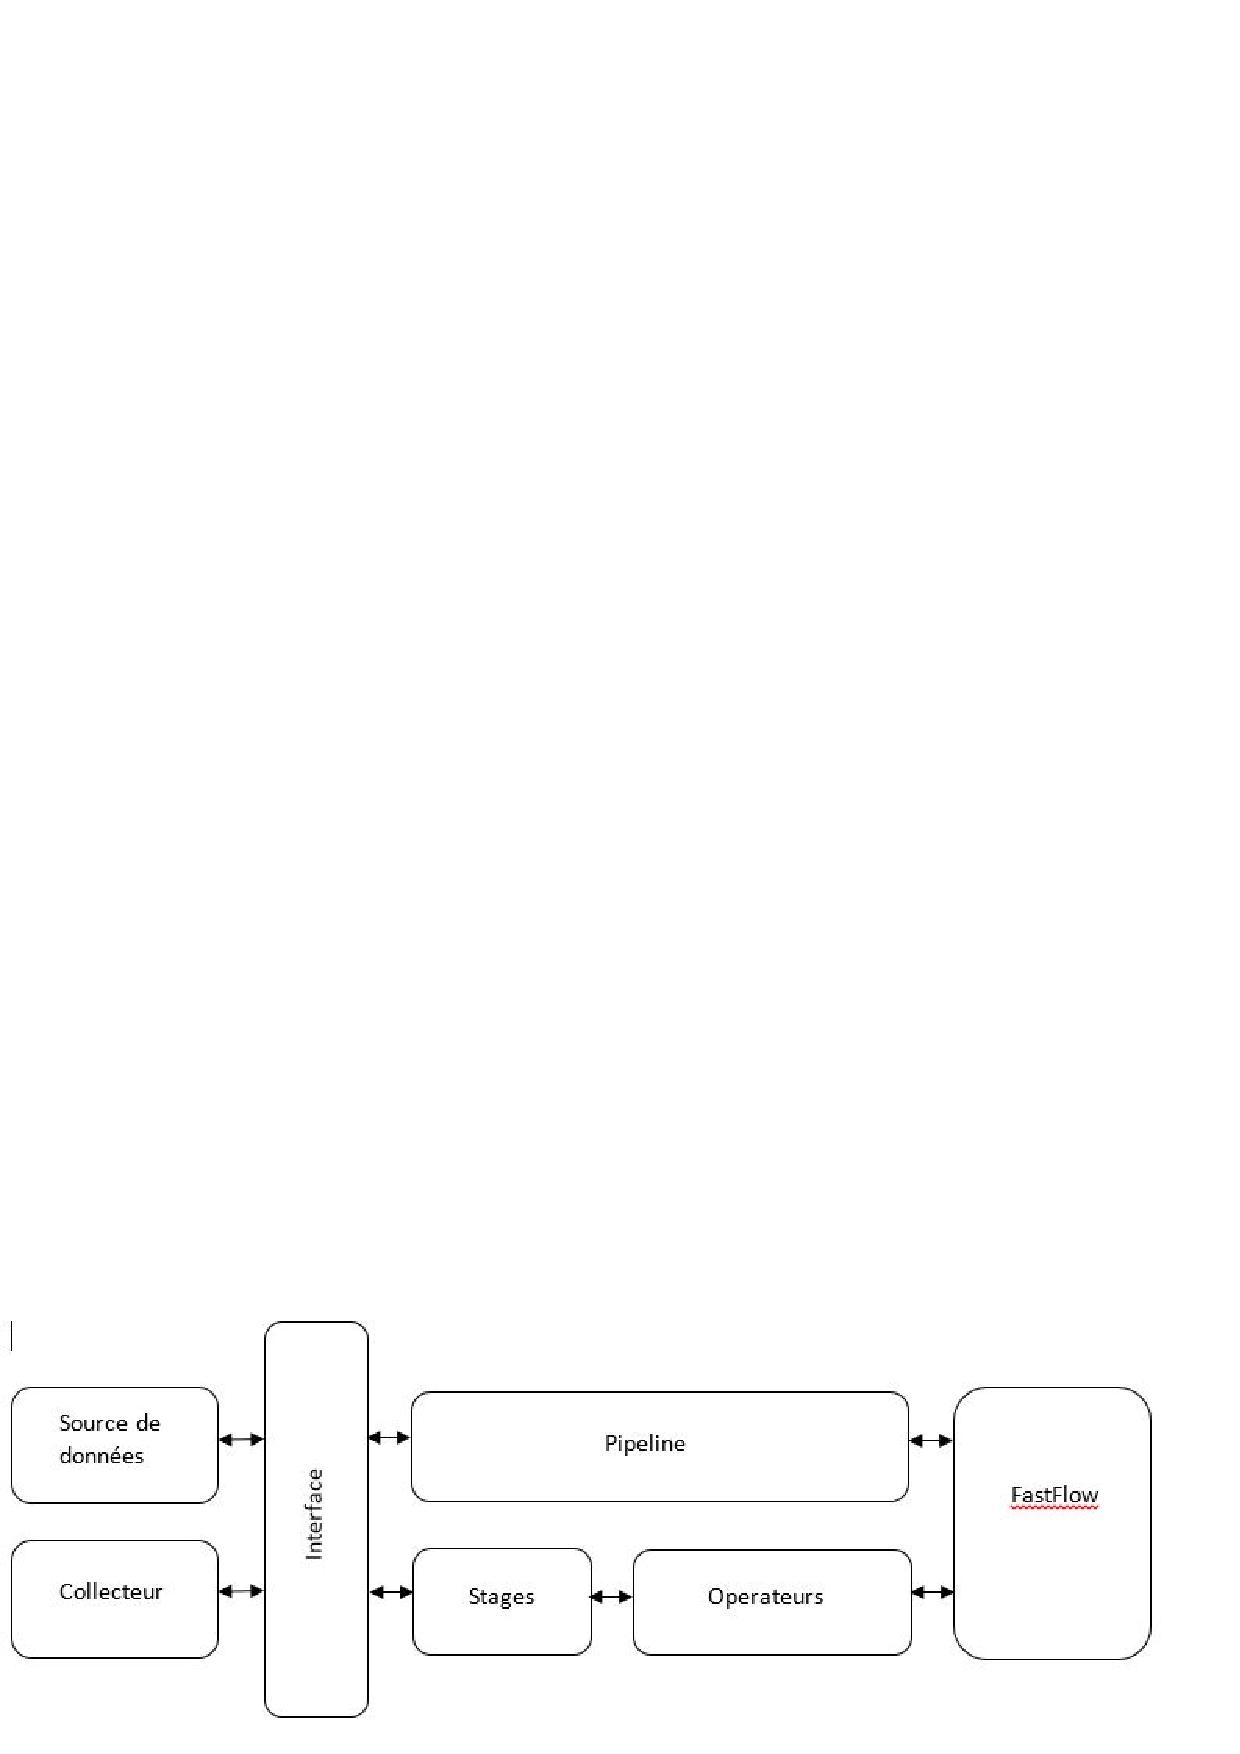
\includegraphics[width=1.0\textwidth]{Figures/ComponentsAPI.jpg}
      \caption{Les composants de l'API de \ppff.}
       \label{ComponentsAPI.fig}
\end{figure}


\gt{Pour ce premier diagramme de classes: il ne faudrait mettre que
les classes qui sont visibles aux utilisateurs, donc les <<concepts>>
qui sont utiles pour utiliser l'API et \^etre capable de s'en
servir. Les autres classes de plus bas niveau (en lien avec FastFlow
par exemple), pourront \^etre pr\'esent\'ees dans le prochain
chapitre.}

\ic{J'ai mis dans le diagramme seulement les classes qui sont visibles aux utilisateurs.}

Ce chapitre pr\'esente l'API de \ppff. Sa conception permet aux utilisateurs de tirer parti de la simplicit\'e d'utilisation tout en cachant la complexit\'e concernant les m\'ecanismes concurrents utilis\'es. La figure~\ref{ComponentsAPI.fig} pr\'esente une vue d'ensemble de l'architecture de \ppff. L'API est compos\'ee de quatre \'el\'ements principaux: l'Interface avec laquelle le d\'eveloppeur interagit, les \TT{Pipeline}s --- qui sont le coeur de l'API ---, les \TT{Stage}s et les \TT{Operator}s. Le r\^ole de chaque composant dans l'API est pr\'esent\'e dans la section suivante. La derni\`ere section  d\'ecrit plus en d\'etail les principales m\'ethodes de l'interface.

\gt{La macro \PpFf{} permet de g\'en\'erer la forme correcte, et
partout pareille. Une version sans majuscule, plus simple \`a
utiliser, produit la m\^eme chose.}

L'{API} de \PpFf{} est impl\'ement\'ee au-dessus de la biblioth\`eque \TT{FastFlow}, impl\'ementation qui sera d\'ecrite au prochain chapitre.

Le pr\'esent chapitre d\'ecrit le r\^ole de chaque composant de
\PpFf{}. La figure~\ref{ClassDiagramme.fig} pr\'esente une vue
d'ensemble des classes qui composent l'{API}.


%\gt{Note que de fa\c{c}on g\'en\'erale, lorsqu'on d\'ebute une section
%qui contient plusieurs sous-sections, il est pr\'ef\'erable d'avoir
%quelques lignes d'introduction, qui donnent une vue d'ensemble de ce
%qui suit. Pas toujours, mais ici, avec le diagramme de classes, \c{c}a
%ferait l'affaire.}
%
%\IC{Mon plan initial \'etait de d\'ecrire les composants dans le chapitre 2 (Description de l'API de \PpFf) et de pr\'esenter la partie technique dans le chapitre 3 (Impl\'ementation). Dans la premi\`ere partie du chapitre 2 j'ai choisi de d\'ecrire les composants principaux de l'API et dans la deuxi\`eme partie de ce chapitre de pr\'esenter quelques m\'ethodes avec des exemples. 
%Dans le chapitre 3 j'ai eu l'intention d'introduire un diagramme de classe UML en expliquant les classes qui compose l'API. } 
%
%\IC{Qu'est-ce que vous en pensez ? Est-ce que je dois introduire le diagramme dans le chapitre 2 ? Je ne suis pas sûr que je fasse la différence entre la description et implémentation de l’API.
%}


%\gt{La description est tout ce qu'un programmeur doit savoir/connaitre
%pour \underline{utiliser} ton API --- de l'ext\'erieur, comme une
%boite noire. L'impl\'ementation d\'ecrit les <<d\'etails>>
%n\'ecessaires pour comprendre \underline{comment fonctionne} l'API,
%par exemple, ce qu'un mainteneur devrait comprendre/connaitre s'il
%voulait modifier, corriger ou \'etendre ton API.}
%
%\gt{En lien avec le diagramme de classes, si l'utilisateur de l'API
%utilise ou manipule diff\'erents concepts et classes dans son
%programme, que ces concepts/classes sont utiles pour pouvoir utiliser
%correctement l'API --- avec la bonne syntaxe et la bonne s\'emantique
%--- alors ces concepts devraient \^etre d\'ecrits, par un diagramme de
%classes par exemple.}


\newpage
\KOMAoptions{paper=landscape,pagesize}
\recalctypearea

\begin{figure}[H]
\centering
     \includegraphics[width=\textwidth]{Figures/ClassDiagramme.jpg}
      \caption{Les classes qui composent l'{API}.}
       \label{ClassDiagramme.fig}
\end{figure}

\newpage
\KOMAoptions{paper=portrait,pagesize}
\recalctypearea



\section{Interface}

L'interface propos\'ee en \PpFf\ consiste en un ensemble de m\'ethodes qui permettent \`a l'utilisateur de manipuler des flux de donn\'ees de mani\`ere simple et efficace. L'interface suit d'assez pr\`es celle introduite pour les \emph{Streams} de Java~8. Le tableau~\ref{methodes_api.tab} d\'ecrit bri\`evement les m\'ethodes impl\'ement\'ees dans l'API.




%\gt{Dans un tabular, pour mettre du texte, on utilise p avec une
%largeur. Ceci \'evite de mettre des sauts de lignes explicites, ce qui
%n'est jamais une bonne id\'ee.}

%\ic{J'ai ajout\'e toutes les m\'ethodes d\'efinies dans l'interface de l'API dans ce tableau et j'ai \'et\'e oblig\'e d'utiliser le paquet longtable parce qu'elle s'\'etendait sur plusieurs pages. J'ai essay\'e de pr\'esenter la signature des m\'ethodes dans un format plus concis. Par exemple le paramètre std ::fonction a \'et\'e remplac\'e pour Func; j'ai enlev\'e les mots typename de chaque d\'eclaration de template; le param\`etre <typename ELEM, class ALLOC = std ::allocator<ELEM class TContainer >> a \'et\'e remplac\'e pour Container. De plus je n'ai pas pu r\'eutiliser la fonction qui redimensionne le tableau resizebox(textwidth). J'ai utilis\'e une police de caract\`ere plus petite (tiny) pour pouvoir encadrer le tableau dans la page.
%}
%
%\IC{J'ai reformul\'e la description pour le r\'esultat de la fonction flatMap}


%\begin{landscape}
\newpage
\KOMAoptions{paper=landscape,pagesize}
\recalctypearea


\begin{center}
\footnotesize
\begin{longtable}{|l|l|p{5cm}|}
\caption{Les m\'ethodes publiques de l'API de~\ppff.\label{methodes_api.tab}}\\
\hline
\textbf{M\'ethode} & \textbf{Type du r\'esultat} & \textbf{Description du r\'esultat}\\
\hline
\endfirsthead
\multicolumn{3}{c}%
{\tablename\ \thetable\ Méthodes publiques de l'API (\textit{suite})} \\
\hline
\textbf{M\'ethode} & \textbf{Type du r\'esultat} & \textbf{Description du r\'esultat}\\
\hline
\endhead
\hline \multicolumn{3}{r}{\textit{Suite page suivante}} \\
\endfoot
\hline
\endlastfoot
\hline
	\begin{tabular}{@{}l@{}}
	\tt template<T> \\
	\tt allMatch(Func<bool(T*)> predicate)
	\end{tabular} &
  	\TT{bool} &
    Retourne \TT{true} si tous les \'el\'ements
    du flux satisfont \TT{predicate}, sinon \TT{false}.
    \\
\hline
	\begin{tabular}{@{}l@{}}
	\tt template<T> \\
	\tt anyMatch(Func<bool(T*)> predicate)
	\end{tabular} &
  	\TT{bool} & 
    Retourne \TT{true} si au moins un  
    \'el\'ement du flux satisfait \TT{predicate}, sinon \TT{false}.
\\
\hline
	\begin{tabular}{@{}l@{}}
	\tt template<T, Container<T>{>}\\
	\tt collect()
	\end{tabular} &
  	\TT{Container<T>} &
    Retourne un conteneur
    STL avec tous les \'el\'ements du flux.
    \\
\hline
	\begin{tabular}{@{}l@{}}
	\tt count()\\
	\end{tabular} &
  	\TT{unsigned int} & 
    Retourne le nombre d'\'el\'ements
    du flux.
    \\
\hline
	\begin{tabular}{@{}l@{}}
	\tt template<In> \\
	\tt find(Func<bool(In*)> const\& predicate)
	\end{tabular} &
  	\TT{Pipe\&} &
    Retourne les
    \'el\'ements du flux qui satisfont \TT{predicate}.
    \\
\hline
	\begin{tabular}{@{}l@{}}
	\tt template<In, Out, Container> \\
	\tt flatMap(Func<Container*(In*)> const\& taskFunc)
	\end{tabular} &
  	\TT{Pipe\&} & 
    Applique la fonction fournie en argument
    \`a chaque \'el\'ement du flux et concat\`ene ces \'el\'ements lorsque plusieurs sont produits par la fonction.
    \\
\hline
	\begin{tabular}{@{}l@{}}
	\tt template<In, Out, Container=In> \\
	\tt flatMap()
	\end{tabular} &
  	\TT{Pipe\&} &
    Produit un flux avec les \'el\'ements du conteneur.  
    \\
\hline
	\begin{tabular}{@{}l@{}}
	\tt template<In, K=In, V=In, MapType> \\
	\tt groupByKey(Func<K*(In*)> fk, Func<V*(In*)> fv)
	\end{tabular} &
  	\TT{MapType} &
    Retourne un dictionnaire (\emph{map}) avec les \'el\'ements
    du flux regroupés par cl\'e.
   \\
\hline
%	\begin{tabular}{@{}l@{}}
%	\tt template<T, Container> \\
%	\tt intermediateCollect()
%	\end{tabular} &
%	\TT{Collection<T, Container>} &
%    Retourne une collection avec les
%    \'el\'ements du flux. 
%    \\ 
%\hline
	\begin{tabular}{@{}l@{}}
	\tt template<T> \\
	\tt limit(int n)
	\end{tabular} &
	\TT{Pipe\&} & 
    Retourne un flux compos\'e des \TT{n}~premiers \'el\'ements du flux d'entr\'ee.
    \\
\hline
	\begin{tabular}{@{}l@{}}
	\tt linesFromFile(string\& path)
	\end{tabular} &
	\TT{Pipe\&} & 
    Retourne un flux avec les lignes
    contenues dans le fichier indiqu\'e par \TT{path}.
    \\
\hline
	\begin{tabular}{@{}l@{}}
	\tt template<In, Out> \\
	\tt map(Func<Out*(In*)> const\& taskFunc)
	\end{tabular} &
	\TT{Pipe\&} & 
    Retourne un flux compos\'e de
    l'application de \TT{taskFunc}
    \`a chacun des
    \'el\'ements du flux.
    \\
\hline
	\begin{tabular}{@{}l@{}}
	\tt template<T> \\
	\tt max(Func<void(T*, T*)> compare)
	\end{tabular} &
	\TT{T} &
	Retourne l'\'el\'ement maximum du flux en fonction du comparateur.
    \\
\hline
	\begin{tabular}{@{}l@{}}
	\tt template<T> \\
	\tt min(Func<void(T*, T*)> compare)
	\end{tabular} &
	\TT{T} &
	Retourne l'\'el\'ement minimum du flux en fonction du comparateur.
    \\
\hline
	\begin{tabular}{@{}l@{}}
	\tt template<T> \\
	\tt noneMatch(Func<bool(T*)> predicate)
	\end{tabular} &
	\TT{bool} &
    Retourne \TT{true} si aucun des \'el\'ements
    du flux ne satisfait \TT{predicate},
    sinon \TT{false}.
    \\
\hline
	\begin{tabular}{@{}l@{}}
	\tt parallel(int workers = 1)
	\end{tabular} &
	\TT{Pipe\&} &
	Sp\'ecifie le nombre de travailleurs \`a utiliser pour traiter les \'el\'ements du flux.
    \\
\hline
	\begin{tabular}{@{}l@{}}
	\tt template<In> \\
	\tt peek(Func<void(In*)> const\& taskFunc)
	\end{tabular} &
	\TT{Pipe\&} &
	Applique la fonction \TT{taskFunc} \`a chaque \'el\'ement du flux et r\'e\'emet l'\'el\'ement (sans le modifier) sur le flux de sortie. Note: Utile pour le d\'ebogage.
    \\
\hline
	\begin{tabular}{@{}l@{}}
	\tt template<In, Out=In> \\
	\tt reduce(Reducer<In, Out> const\& reducer)
	\end{tabular} &
	\TT{Out} &
	Effectue une r\'eduction sur les \'el\'ements du flux. Voir la notion de \TT{reducer}, p.~\pageref{reducer.sect}.
    \\
\hline
	\begin{tabular}{@{}l@{}}
	\tt template<In, Out=In> \\
	\tt reduce(Out init, Func<Out(In, Out)> acc)
	\end{tabular} &
	\TT{Out} &
	Effectue une r\'eduction des \'el\'ements du flux, en utilisant \TT{init} comme valeur initiale et \TT{acc} comme fonction d'accumulation.
    \\
\hline
	\begin{tabular}{@{}l@{}}
	\tt template<In, K=In, V=In, MapType> \\
	\tt reduceByKey(Reducer<In, V> r, Func<K*(In*)> fk)
	\end{tabular} &
	\TT{MapType} &
    Effectue une r\'eduction sur les valeurs de chaque cl\'e à l'aide d'op\'erateur \TT{Reducer}. Voir la notion de \TT{Reducer}, p.~\pageref{reducer.sect}.
    \\
\hline
	\begin{tabular}{@{}l@{}}
	\tt template<T> \\
	\tt skip(int n)
	\end{tabular} &
	\TT{Pipe\&} &
    Retourne un flux compos\'e des \'el\'ements du flux d'entr\'ee, mais en omettant les \TT{n} premiers \'el\'ements.
    \\
\hline
	\begin{tabular}{@{}l@{}}
	\tt template<T> \\
	\tt sort(Func<bool(T, T)> const\& compare)
	\end{tabular} &
	\TT{Collection<T, Container>} &
	Effectue le tri des \'el\'ements du flux, selon l'ordre sp\'ecifi\'e par \TT{compare}. Note: Le premier \'el\'ement du flux de sortie n'est \'emis \emph{qu'apr\`es que la fin de flux ait \'et\'e rencontr\'ee}.
    \\
\hline
	\begin{tabular}{@{}l@{}}
	\tt template<T, Iterator> \\
	\tt source(Iterator  begin, Iterator end)
	\end{tabular} &
	\TT{Pipe\&} &
	Convertit un conteneur de type {STL} en flux.
    \\
\hline
	\begin{tabular}{@{}l@{}}
	\tt template<T> \\
	\tt sum()
	\end{tabular} &
	\TT{T} &
	Retourne la somme des \'el\'ements du flux.
    \\
\hline
\end{longtable}
\normalsize
\end{center}




%\end{landscape}
\newpage
\KOMAoptions{paper=portrait,pagesize}
\recalctypearea







%\begin{table}[h]
%\centering
%
%\resizebox{\textwidth}{!}{%
%
%\begin{tabular}{|l|l|p{8cm}|}
%\hline
%\textbf{M\'ethode} & \textbf{Type du r\'esultat} & \textbf{Description du r\'esultat}\\
%\hline
%	\begin{tabular}{@{}l@{}}
%	\tt template<T> \\
%	\tt allMatch(Func<bool(T*)> predicate)
%	\end{tabular} &
%  	\TT{bool} &
%    Retourne \TT{true} si tous les \'el\'ements
%    du flux correspondent au pr\'edicat
%    fourni, sinon \texttt{false}.
%    \\
%\hline
%	\begin{tabular}{@{}l@{}}
%	\tt template<T> \\
%	\tt anyMatch(Func<bool(T*)> predicate)
%	\end{tabular} &
%  	\texttt{bool} & 
%    Retourne \texttt{true} si au moins un  
%    \'el\'ement du flux correspondent
%    au pr\'edicat fourni, sinon \texttt{false}.
%\\
%\hline
%	\begin{tabular}{@{}l@{}}
%	\tt template<T, Container<T>>\\
%	\tt collect()
%	\end{tabular} &
%  	\texttt{Container<T>} &
%    Retourne un conteneur de type
%    STL contenant les \'el\'ements du flux.
%    \\
%\hline
%	\begin{tabular}{@{}l@{}}
%	\tt count()\\
%	\end{tabular} &
%  	\texttt{unsigned int} & 
%    Retourne le nombre d'\'el\'ements
%    dans ce flux.
%    \\
%\hline
%	\begin{tabular}{@{}l@{}}
%	\tt template<In> \\
%	\tt find(Func<bool(In*)> const\& taskFunc)
%	\end{tabular} &
%  	\texttt{Pipe\&} &
%    Retourne tous les
%    \'el\'ements du flux qui satisfont la 
%    fournie en argument.
%    \\
%\hline
%	\begin{tabular}{@{}l@{}}
%	\tt template<In, Out, Container> \\
%	\tt flatMap(Func<Container*(In*)> const\& taskFunc)
%	\end{tabular} &
%  	\texttt{Pipe\&} & 
%    Applique la fonction fournie en argument
%    \`a chaque \'el\'ement du flux.
%    \\
%\hline
%	\begin{tabular}{@{}l@{}}
%	\tt template<In, Out, Container=In> \\
%	\tt flatMap()
%	\end{tabular} &
%  	\texttt{Pipe\&} &
%    \GT{Reformuler: je ne comprends pas la diff\'erence avec le pr\'ec\'edent}    
%    \\
%\hline
%	\begin{tabular}{@{}l@{}}
%	\tt template<In, K=In, V=In, MapType> \\
%	\tt groupByKey(Func<K*(In*)> fk, Func<V*(In*)> fv)
%	\end{tabular} &
%  	\texttt{MapType} &
%    Retourne un dictionnaire (\emph{map}) avec les \'el\'ements
%    du flux regroupés par cl\'e.
%   \\
%\hline
%	\begin{tabular}{@{}l@{}}
%	\tt template<T, Container> \\
%	\tt intermediateCollect()
%	\end{tabular} &
%	\texttt{Collection<T, Container>} &
%    Retourne une collection avec les
%    \'el\'ements du flux.
%    \\ 
%\hline
%	\begin{tabular}{@{}l@{}}
%	\tt template<T> \\
%	\tt limit (int n)
%	\end{tabular} &
%	Pipe\& & 
%    Renvoie dans le flux seulement
%    les n premiers \'el\'ements de
%    ce flux.
%    \\
%\hline
%	\begin{tabular}{@{}l@{}}
%	\tt linesFromFile(string\& path)
%	\end{tabular} &
%	Pipe\& & 
%    Renvoie dans le flux les lignes
%    contenues dans un fichier.
%    \\
%\hline
%	\begin{tabular}{@{}l@{}}
%	\tt template<In, Out> \\
%	\tt map(Func<Out*(In*)> const\& taskFunc)
%	\end{tabular} &
%	Pipe\& &
%    Renvoie dans le flux les
%    r\'esultats constitu\'es de 
%    l'application d'une fonction 
%    fournie en param\`etre aux 
%    \'el\'ements du flux.
%    \\
%\hline
%	\begin{tabular}{@{}l@{}}
%	\tt template<T> \\
%	\tt max(Func<void(T*, T*)> compare)
%	\end{tabular} &
%	\texttt{T} &
%	Retourne l'\'el\'ement maximum du flux en fonction du comparateur fourni en param\`etre.
%    \\
%\hline
%	\begin{tabular}{@{}l@{}}
%	\tt template<T> \\
%	\tt min(Func<void(T*, T*)> compare)
%	\end{tabular} &
%	\texttt{T} &
%	Retourne l'\'el\'ement minimum du flux en fonction du comparateur fourni en param\`etre.
%    \\
%\hline
%	\begin{tabular}{@{}l@{}}
%	\tt template<T> \\
%	\tt noneMatch(Func<bool(T*)> predicate)
%	\end{tabular} &
%	\texttt{bool} &
%	Retourne l'\'el\'ement minimum du flux en fonction du comparateur fourni en param\`etre.
%    \\
%\hline
%	\begin{tabular}{@{}l@{}}
%	\tt parallel(int workers = 1)
%	\end{tabular} &
%	Pipe\& &
%	D\'efinis le nombre de travailleurs fourni en param\`etre.
%    \\
%\hline
%	\begin{tabular}{@{}l@{}}
%	\tt template<In> \\
%	\tt peek(Func<void(In*)> const\& taskFunc)
%	\end{tabular} &
%	Pipe\& &
%	M\'ethode utilis\'ee pour d\'ebogage. Applique une fonction sur les \'el\'ements du flux sans modifier leur valeur.
%    \\
%\hline
%	\begin{tabular}{@{}l@{}}
%	\tt template<In, Out=In> \\
%	\tt reduce(Reducer<In, Out> const\& reducer)
%	\end{tabular} &
%	\texttt{Out} &
%	reduce description.
%    \\
%\hline
%	\begin{tabular}{@{}l@{}}
%	\tt template<In, Out=In> \\
%	\tt reduce(Out init, Func<Out(In, Out)> acc)
%	\end{tabular} &
%	\texttt{Out} &
%	reduce description.
%    \\
%\hline
%	\begin{tabular}{@{}l@{}}
%	\tt template<In, K=In, V=In, MapType> \\
%	\tt reduceByKey(Reducer<In, V> r, Func<K*(In*)> fk)
%	\end{tabular} &
%	\texttt{MapType} &
%	reduceByKey description.
%    \\
%\hline
%	\begin{tabular}{@{}l@{}}
%	\tt template<T> \\
%	\tt skip(int n)
%	\end{tabular} &
%	Pipe\& &
%	skip description.
%    \\
%\hline
%	\begin{tabular}{@{}l@{}}
%	\tt template<T> \\
%	\tt sort(Func<bool(T, T)> const\& compare)
%	\end{tabular} &
%	\texttt{Collection<T, Container>} &
%	sort description.
%    \\
%\hline
%	\begin{tabular}{@{}l@{}}
%	\tt template<T, Iterator> \\
%	\tt source(Iterator  begin, Iterator end)
%	\end{tabular} &
%	Pipe\& &
%	source description.
%    \\
%\hline
%	\begin{tabular}{@{}l@{}}
%	\tt template<T> \\
%	\tt sum()
%	\end{tabular} &
%	\texttt{T} &
%	sum description.
%    \\
%\hline
%
%
%\end{tabular}
%}
%\caption{Les m\'ethodes expos\'ees aux utilisateurs par l'API de \ppff.}
%\label{methodes_api.tab}
%\end{table}




Comme on peut le voir dans le tableau~\ref{methodes_api.tab}, la d\'eclaration des m\'ethodes utilise la programmation g\'en\'erique de C++, c'est-\`a-dire les \emph{templates}. Cela permet aux utilisateurs d'avoir une interface g\'en\'erique unique, de sorte qu'une m\'ethode peut \^etre r\'eutilis\'ee pour n'importe quel type de donn\'ees.


Un autre point cl\'e dans cette interface est son expressivit\'e. M\^eme avant sa conception d\'etaill\'ee, nous nous \'etions donn\'es comme objectif de fournir un syst\`eme suffisamment intuitif et expressif pour le traitement de flux de donn\'ees. 

\gt{Lorsque dans le texte tu indiques des identificateurs qui viennent du code --- find, collect, etc. --- alors il faut les mettre en police tt, donc \TT{find}, \TT{collect}, etc.}


\gt{Comme indiqu\'e dans le chapitre pr\'ec\'edent, oublie ce que
j'avais \'ecrit concernant l'environnement Listing, car cela ne
produit pas le bon num\'ero, tel qu'officiellement requis par le guide
UQAM (2.1, 2.2, etc.).  Il faut plut\^ot utiliser les diverses options
associ\'ees directement \`a lstlisting. Pour rappel, voir le chapitre
pr\'ec\'edent ainsi que l'exemple de Reducer un peu plus bas.}


\ic{J'ai v\'erifi\'e le terme listing dans tout le document. Vous les avez remplac\'es par tout. }


%
% Tu as deja ce listing plus bas!?
% \begin{lstlisting}[
% label={reducer.c++},
% language=c++,
% caption={La signature d'un objet \TT{Reducer}.},
% frame=single,
% float]
%  template<typename In, typename Out>
%  class Reducer {
%        Reducer(Out init, 
%                Func<Out(Out, In)> const& accumulator,
%                Func<Out(Out, Out)> const& combiner)

%        Reducer(Func<Out(Out, In)> const& accumulator,
%                Func<Out(Out, Out)> const& combiner)

%        Reducer(Out init, 
%                Func<Out(Out, In)> const& accumulator)
%  }
% \end{lstlisting}


\begin{lstlisting}[
label={expressivite_api.c++},
language=c++,
caption={Un exemple illustrant les principaux \'el\'ements de l'API de \ppff.},
frame=single,
float]
// Definition (omise) d'un vecteur d'objets Employee.
std::vector<Employee> sourceEmployees;
...

std::vector<Employee> result = 
   Pipe()
   .source<Employee>(sourceEmployees.begin(), sourceEmployees.end())
   .find<Employee>([](Employee *e) { return e->salary > 35000; })
   .collect<Employee, std::vector>();
\end{lstlisting}




Le listing~\ref{expressivite_api.c++} pr\'esente un extrait de code C++ qui donne un premier aper\c{c}u de l'expressivit\'e de l'interface --- d'autres exemples seront pr\'esent\'es plus loin. Dans cet exemple, on s\'electionne les employ\'es qui ont un salaire plus grand que 35~K\$. Les employ\'es sont initialement dans un conteneur STL et sont filtr\'es en chainant trois op\'erations : $i)$ \TT{source} qui permet d'envoyer dans le flux des objets de type~\TT{Employe}; $ii$) \TT{find} qui s\'electionne les employ\'es selon la condition fournie en param\`etre (une lambda-expression); $iii)$ \TT{collect} qui met les employ\'es s\'electionn\'es dans un conteneur STL. Ici, les employ\'es s\'electionn\'es sont mis dans un conteneur de type \TT{std::vector} --- le type de conteneur est donn\'e par le type fourni en argument (g\'en\'erique) de la m\'ethode \TT{collect}.




\section{Op\'erateurs}

Les op\'erateurs (classe \TT{Operator}) sont la base de notre syst\`eme. L'API fournit un ensemble d'op\'erateurs qui facilitent la t\^ache de l'utilisateur. Les op\'erateurs sont structur\'es en deux cat\'egories : les op\'erateurs sans \'etat et les op\'erateurs avec \'etat.

Les \emph{op\'erateurs sans \'etat} sont ceux qui ne disposent pas d'informations sur l'it\'eration en cours et ne transmettent pas les informations interm\'ediaires des \'etapes de traitement pr\'ec\'edentes. Si on prend comme exemple le filtre repr\'esent\'e par la m\'ethode \TT{find} du tableau~\ref{methodes_api.tab}, il traite le flux de donn\'ees \'el\'ement par \'el\'ement. 
%
Lorsque la fonction (lambda-expression) fournie en argument \`a la m\'ethode \TT{find} ne satisfait pas la condition lorsqu'appliqu\'ee \`a un \'el\'ement du flux, le filtre ne retourne rien. 

Les \emph{op\'erateurs avec \'etat} sont ceux qui maintiennent une structure de donn\'ees interne, qui repr\'esente l'\'etat. Cette structure repr\'esente ou synth\'etise l'historique des \'el\'ements pass\'es au flux et affecte la logique de traitement dans les calculs ult\'erieurs. Par exemple, l'op\'erateur \TT{Sum} calcule la somme des \'el\'ements du flux. Son \'etat contient la valeur de la somme de tous les \'el\'ements qui pr\'ec\'edent celui en cours de traitement. 

\subsection*{Op\'erateurs de r\'eduction}

\label{reducer.sect}

\begin{lstlisting}[
label={reducer.c++},
gobble=1,
language=c++,
caption={La signature d'un objet \TT{Reducer}.},
frame=single,
float]
 template<typename In, typename Out>
 class Reducer {
       Reducer(Out init, 
               Func<Out(Out, In)> const& accumulator,
               Func<Out(Out, Out)> const& combiner)

       Reducer(Func<Out(Out, In)> const& accumulator,
               Func<Out(Out, Out)> const& combiner)

       Reducer(Out init, 
               Func<Out(Out, In)> const& accumulator)
 }
\end{lstlisting}



\gt{Une règle utile à savoir pour \LaTeX: lorsqu'on met un élément
flottant (avec caption/label, e.g., figure, table, pseudocode,
listing), il est préférable de mettre cet élément \underline{avant} la
première référence (et non pas après).  La position du flottant par
rapport au texte qui y réfère est alors meilleure.}

L'op\'erateur de classe \TT{Reducer} est utilis\'e pour r\'eduire les \'el\'ements du flux \`a une valeur unique. Le listing~\ref{reducer.c++} présente la spécification  de la classe \TT{Reducer} avec les signatures des fonctions associées. 


\begin{lstlisting}[
label={sumElementsCollectionWithReducer},
language=c++,
gobble=4,
caption={[Exemple d'utilisation de l'opérateur \TT{Reducer}.]Exemple
d'utilisation de l'opérateur \TT{Reducer}~: ici, les \'el\'ements
d'une collection sont simplement additionn\'es entre eux, avec
l'op\'erateur \TT{std::plus<int>\{\}}.},
frame=single,
float]
    int n = 100;
    std::vector<int> elems(n);
    for (unsigned int i = 0; i < elems.size(); i++) {
        elems[i] = i;
    };

    Reducer<int, int> reducer(std::plus<int>{});

    int currentResult =
        Pipe()
        .source<int>(elems.begin(), elems.end())
        .reduce<int, int>(reducer);

	std::cout << "Result: " << currentResult;	// == 4950   
\end{lstlisting}



Un \TT{Reducer} est construit avec une valeur initiale, une fonction \TT{accumulator} et une fonction \TT{combiner}. La valeur initiale et la fonction \TT{combiner} sont optionnelles gr\^ace \`a la surcharge du constructeur. Lorsque ces arguments sont omis, la valeur initiale est initialis\'ee \`a la valeur par d\'efaut du type de cette valeur et la fonction \TT{combiner} est remplac\'ee par la fonction \TT{accumulator}. Par exemple, le listing~\ref{sumElementsCollectionWithReducer} montre un exemple d'utilisation de l'op\'erateur \TT{Reducer}. La valeur initiale est sp\'ecifi\'ee comme \'etant \TT0 et la fonction \TT{combiner} est indiqu\'ee par la fonction d'addition \TT{std::plus<int>\{\}}. 


\begin{lstlisting}[
label={sumElementsCollectionWithReducerParallel},
gobble=4,
language=c++,
caption={[Exemple d'utilisation de l'opérateur \TT{Reducer}, ex\'ecut\'e en
parall\`ele et avec une valeur initiale.]Exemple
d'utilisation de l'opérateur \TT{Reducer}, ex\'ecut\'e en parall\`ele et avec une
valeur initiale non nulle sp\'ecifi\'ee explicitement.},
frame=single,
float]
    int n = 100;
    std::vector<int> elems(n);
    for (unsigned int i = 0; i < elems.size(); i++) {
        elems[i] = i;
    };

    // Avec valeur initiale explicite... pour illustrer l'effet!
    Reducer<int, int> reducer(3, 
                              std::plus<int>{}, 
                              std::plus<int>{});

	int currentResult =
		Pipe()
		.source<int>(elems.begin(), elems.end())
		.parallel(2)
		.reduce<int, int>(reducer); 
	
	std::cout << "Result: " << currentResult;	// == 4953
\end{lstlisting}




Le troisi\`eme param\`etre de l'op\'erateur \TT{Reducer}, la fonction \TT{combiner}, est utilis\'ee lorsque le flux est trait\'e en parall\`ele, par plusieurs \emph{threads}. Dans un tel cas, le flux est divis\'e en sous-flux --- i.e., chaque \emph{thread} traite un sous-ensembles des éléments --- qui sont r\'eduits en parall\`ele avec la fonction \TT{accumulator}. Les r\'esultats partiels produits par les divers \emph{threads} sont ensuite combin\'es, dans le \emph{thread} principal, avec la fonction \TT{combiner}. Le listing~\ref{sumElementsCollectionWithReducerParallel} montre un exemple d'utilisation de l'op\'erateur \TT{Reducer} mais ex\'ecut\'e en parall\`ele. Dans cet exemple, \`a des fins d'illustration, une valeur initiale est sp\'ecifi\'ee, \'egale \`a \TT3 et, alors que les fonctions \TT{combiner} et \TT{accumulator} sont toutes deux indiqu\'ees comme \'etant la fonction d'addition \TT{std::plus<int>\{\}}. 


\gt{R\'esultat incorrect indiqu\'e je crois: 4953 => 5053!?}

\ic{J’ai pris l’exemple des tests unitaires. La formule de calcul pour
le résultat attendu est~:  expectedResult = n * (n - 1) / 2;}

\GT{L'exemple ne semble pas \^etre le m\^eme: \TT{elems[i] = i+1} vs.\
\TT{elems[i] = i} comme dans l'exemple pr\'ec\'edent, donc r\'esultats
diff\'erents. J'ai corrig\'e/adapt\'e pour avoir le m\^eme exemple,
donc le m\^eme r\'esultat, modulo la valeur initiale!}

\section{Pipeline}


\begin{figure}[ht]
\centering
     \includegraphics[width=1.0\textwidth]{Figures/Pipeline.jpg}
      \caption[Repr\'esentation graphique d'un pipeline.]{Une repr\'esentation graphique d'un pipeline. \GT{Donner des explications additionnelles~: voir plus bas.}}
       \label{Pipeline.fig}
\end{figure}


Le \TT{Pipeline} est le composant principal de notre {API}. Un \TT{Pipeline} est une cha\^{\i}ne de traitement compos\'ee d'un ou plusieurs \TT{Operator}s regroup\'es dans des \TT{Stages}. La figure~\ref{Pipeline.fig} montre une vue d\'etaill\'ee d'un \TT{Pipeline} en action. Une \'etape de la cha\^{\i}ne de traitement de ce mod\`ele traite les donn\'ees produites par l'\'etape pr\'ec\'edente dans le flux et fournit les r\'esultats \`a l'étape suivante dans le flux. Un pipeline \TT{P} avec $n$ \'etapes peut \^etre d\'efini comme suit:


\[
	\TT{P} = O_1 +  \ldots + O_k + \ldots + O_n
\]


Dans l'expression ci-dessus, $O_k$ d\'enote le $k^e$ op\'erateur dans le pipeline~\TT{P}.


\GT{Il faut clarifier la partie ci-haut. On ne comprends pas pourquoi
$P = O_1 + \ldots + O_n$ --- pourquoi <<+>>? Pourquoi ne pas utiliser
le symbole de pipe comme en Unix, i.e., <<$\vert$>>?  Ce serait plus
naturel peut-\^etre?  (Parce que dans plusieurs notations formelles,
<<+>> est utilis\'e pour repr\'esenter un {\bf choix}, et non une
s\'equence cons\'ecutive d'items.)}

\GT{En outre, on ne comprend pas le lien entre cette \'equation et la
figure.  Ce serait pr\'ef\'erable qu'on puisse comprendre quel est
exactement ce qui est repr\'esent\'e par la figure: il y a un premier
pipeline s\'equentiel, form\'e de 3 op\'erateurs, un autre parall\`ele
(form\'e de 4 op\'erateurs), puis un autre (de 2 op\'erateurs).
Sinon, on cherche \`a comprendre \`a quoi la figure correspond, quel
est le lien avrc l'\'equation. Parce qu'en ce moment, il me semble que
l'\'equation n'est pas utile --- elle le serait si elle \'etait
ensuite utilis\'ee plus loin, ailleurs, pour expliquer/repr\'esenter
autre chose, ce qui n'est pas le cas.}



L'utilisation de \TT{Pipeline} introduit une couche d'abstraction sur une cha\^{\i}ne complexe d'op\'erateurs. De plus, un \TT{Pipeline} n'expose à l'ext\'erieur que ses entr\'ees et ses sorties. Une telle conception modulaire permet une flexibilit\'e au syst\`eme tout en simplifiant la mise en œuvre. Par exemple, le parall\'elisme de donn\'ees
pourrait \^etre facilement r\'ealis\'e en ayant plusieurs \TT{Pipeline}s identiques connect\'es \`a la m\^eme entr\'ee et sortie respectivement.


\section{Travailler avec des flux}

Cette section pr\'esente de fa\c{c}on plus d\'etaill\'ee quelques-unes des m\'ethodes disponibles dans \PpFf. Elle pr\'esente \'egalement le code source d'un petit exemple, \TT{WordCount}, pour illustrer l'utilisation de l'API et l'effet des principales op\'erations. 

Utiliser des flux dans \PpFf{} implique de d\'efinir et combiner trois \'el\'ements: 
\begin{itemize}
	\item Une source de donn\'ees --- par ex., une collection --- pour produire les \'el\'ements initiaux du flux;

	\item Une cha\^ine d'op\'erations, sans \'etat, qui forment un pipeline;

	\item Une op\'eration avec \'etat qui d\'eclenche l'ex\'ecution des op\'erations du flux pour produire un r\'esultat.
\end{itemize}


\begin{lstlisting}[
label={wordcount.c++},
language=c++,
caption={Le code source d'une application pour compter le nombre d'occurrences de mots dans un texte.},
frame=single,
float]
typedef std::vector<std::string> Words;

bool notEmpty(std::string* s) { return s->size() > 0; }

int main(int argc, char* argv[]) {
  Reducer<std::string, int> sumOccurrences(
    0, 
    [](int count, std::string _) { return count + 1; },
    std::plus<int>{} );

  std::string path = "/home/Words.txt"; 

  std::unordered_map<std::string, int> currentResult = 
	Pipe()
    .linesFromFile(path) 
    .parallel(4)
    .flatMap<std::string, std::string, Words>(splitInWords)
    .map<std::string, std::string>(toLowercaseLetters)
    .find<std::string>(notEmpty)
    .reduceByKey<std::string, std::string, int>(sumOccurrences);
}
\end{lstlisting}




Pour illustrer un flux dans \PpFf, le listing~\ref{wordcount.c++} montre le code source d'une petite application pour compter le nombre d'occurrences des mots dans un fichier texte. Une telle application est compos\'ee de plusieurs \'etapes. 

La premi\`ere \'etape d\'efinit la source du flux. Dans l'application de compte de mots, la source est constitu\'ee par les lignes contenues dans un fichier. C'est la m\'ethode \TT{linesFromFile(path)} qui permet d'extraire et retourner dans le flux les lignes du fichier. Le fichier est sp\'ecifi\'e par la variable \TT{path} fournie en argument \`a la m\'ethode \TT{linesFromFile}. 

Dans notre exemple, la deuxi\`eme \'etape dans l'application de compte de mots est l'appel \`a \TT{parallel}. Ceci permet de partitionner les \'el\'ements du flux entre divers \emph{threads} --- ici, quatre (4) \emph{threads} --- et donc d'ex\'ecuter les \'etapes qui suivent en parall\`ele. 

Les op\'erations subs\'equentes du pipeline sont les suivantes :
\begin{itemize}

\item L'op\'eration \TT{flatMap} d\'ecompose chaque ligne en mots individuels en appliquant la fonction \TT{splitInWords} sur chacune des lignes;

\item L'op\'eration \TT{map} transforme chacun des mots en rempla\c{c}ant les lettres majuscules d'un mot en lettres minuscules en appliquant la fonction \TT{toLowerCaseLetters}.

\item L'op\'eration \TT{find} retourne dans le flux seulement les mots qui ne sont pas vides (\TT{notEmpty}).


% \gt{Lorsqu'on utilise des tirets explicatifs, i.e., <<--->>, il faut
% mettre trois tirets et, en fran\c{c}ais, il faut laisser un espace
% avant et apr\`es les trois tirets.}

\item Finalement, l'op\'eration \TT{reduceByKey}  regroupe les mots similaires ensemble et compte le nombre d'occurrences de chaque mot, et ce par l'utilisation du \TT{Reducer} \TT{sumOccurrences}. 
\end{itemize}





\subsection{Le flux}


Un programme \PpFf{} est un ensemble d'objets de type \TT{Operator} compos\'es dans un objet de type flux. Au niveau utilisateur, un flux est repr\'esent\'e par une instance de la classe \TT{Pipe} --- voir la figure~\ref{ClassDiagramme.fig}. 


Un flux est ex\'ecut\'e en parall\`ele lorsqu'un appel \`a la m\'ethode \TT{parallel} est ajout\'e dans la chaine d'op\'erations. Le param\`etre optionnel de cette m\'ethode d\'efinit le nombre de travailleurs \`a utiliser pour l'ex\'ecution parall\`ele. Par exemple, un appel tel que \TT{parallel(4)} dans le programme du d\'ecompte du nombre de mots du listing~\ref{wordcount.c++} indique qu'il faut ex\'ecuter en parall\`ele toutes les op\'erations suivant cette m\'ethode;  le nombre de travailleurs utilis\'es dans ce cas est quatre. Si ce param\`etre n'est pas fourni,  un seul travailleur est utilis\'e par d\'efaut. 


\begin{lstlisting}[
label={wordcountParallel.c++},
language=c++,
caption={Un autre pipeline pour compter les mots, mais un nombre de travailleurs qui varie selon les \'etapes du pipeline.},
frame=single,
float]
std::unordered_map<std::string, int> currentResult = 
	Pipe()
	.linesFromFile(path) 
	.flatMap<std::string, std::string, Words>(splitInWords)
	.parallel(4)
	.map<std::string, std::string>(toLowercaseLetters)
	.find<std::string>(notEmpty)
	.parallel(2)
	.reduceByKey<std::string, std::string, int>(reducer);
\end{lstlisting}




\PpFf{} est assez flexible en permettant l'ex\'ecution des op\'erations en parall\`ele avec un nombre diff\'erent de travailleurs. Par exemple, dans le listing~\ref{wordcountParallel.c++}, l’opération \TT{flatMap} du programme de d\'ecompte du nombre de mots est exécutée avec un seul travailleur, les opérations \TT{map} et \TT{find} sont exécutées avec quatre travailleurs et la dernière opération, \TT{reduceByKey}, avec deux travailleurs. 


% \gt{Les mots qui correspondent \`a des noms de m\'ethodes ou des
% \'el\'ements du code (par ex., variables, etc., doivent \^etre mis en
% police texttt.  C'est ce que fait la macro TT, que j'ai d\'efinie.}

% \gt{Dans une phrase, les nombres plus petits que 10 sont
% g\'en\'eralement mis en mots, plut\^ot qu'en chiffres. }


% Les op\'erateurs sont ajout\'es dans le flux simplement en encha\^inant les m\'ethodes d\'esir\'ees. Par exemple, toujours dans le programme du d\'ecompte du nombre de mots du listing~\ref{wordcountParallel.c++}, la m\'ethode \TT{map} ajoute l'opérateur \TT{Map} et la m\'ethode \TT{find} ajoute l'op\'erateur \TT{Find}. 

% Deja dit plus haut, donc inutile de repeter.
% Les sous-sections suivantes pr\'esentent une description compl\`ete de quelques m\'ethodes impl\'ement\'ees dans l'interface.


\subsection{Source}

La source de donn\'ees est le premier op\'erateur ajout\'e dans un flux. Sans un tel op\'erateur, un flux ne peut pas \^etre ex\'ecut\'e puisqu'il n'y a pas de donn\'ees \`a traiter. 

L'API fournit des m\'ethodes pour \'emettre des donn\'ees \`a partir de diverses sources, telles que des collections ou des fichiers. Des travaux futurs pourraient \'etendre l'interface pour prendre en charge plus des sources de donn\'ees. 


\gt{Attention: dans un m\^eme paragraphe, tu m\'elanges la
pr\'esentation g\'en\'erale --- telle que donn\'ee dans le tableau ---
et un exemple sp\'ecifique.  Tu peux faire les deux, mais je sugg\`ere
de bien distinguer entre les deux dans ce cas: un paragraphe qui
pr\'esente l'id\'ee/forme g\'en\'erale; un autre paragraphe qui
illustre concr\`etement avec un exemple.}

\ic{J'ai cr\'e\'e deux paragraphes.}

Les signatures pour les deux m\'ethodes sont donn\'ees dans le tableau~\ref{methodes_api.tab}. Tandis que la premi\`ere m\'ethode, \TT{linesFromFile}, consomme les donn\'ees \`a partir d'un fichier, la deuxi\`eme m\'ethode, \TT{source}, consomme les donn\'ees \`a partir d'un conteneur STL.


\begin{lstlisting}[
label={mapExample.c++},
language=c++,
caption={Transformation d'une collection d'entiers en un autre collection d'entiers en appliquant une lambda-expression sur chacun des \'el\'ements.},
frame=single,
float]
std::vector<int> elems = {0, 1, 2, 3, 4, 5, 6, 7, 8, 9};

std::vector<int> currentResult =
    Pipe()
    .source<int>(elems.begin(), elems.end())
    .map<int, int>( [](int *in){ *in *= 3; return in; } )
    .collect<int, std::vector>();            
\end{lstlisting}




Les deux m\'ethodes d'entr\'ee dans le flux sont illustr\'ees dans les exemples du listing~\ref{wordcount.c++} et respectivement~\ref{mapExample.c++}. La m\'ethode, \TT{linesFromFile} du listing~\ref{wordcount.c++} envoie dans le flux chaque ligne du fichier \TT{Words.txt}. Le param\`etre \TT{path} sp\'ecifie le chemin o\`u se trouve le fichier. Dans le deuxième exemple fourni dans le listing~\ref{mapExample.c++}, les donn\'ees sont consomm\'ees \`a partir de \TT{elems}, un \TT{vector}. La m\'ethode \TT{source} envoie dans le flux les donn\'ees de type \TT{int} en fournissant les it\'erateure de d\'ebut et fin du \TT{vector elems}.


\subsection{Map}

% \gt{Dans un texte scientifique, dont un m\'emoire, on utilise <<nous>>
% assez rarement. En fait, on utilise <<nous>> surtout comme une
% fa\c{c}on plus formelle de dire <<je>>.  Voir:
% \url{https://fr.wiktionary.org/wiki/nous_de_modestie}}


\begin{lstlisting}[
label={mapExample2.c++},
language=c++,
caption={S\'election des noms de tous les employ\'es d'une collection.},
frame=single,
float]
std::vector<std::string> result =
    Pipe()
    .source<Employee>(elems.begin(), elems.end())
    .map<Employee, std::string>( [](Employee *e) 
                                   { return &(e->getName()); } )
    .collect<std::string, std::vector>();
\end{lstlisting}




La m\'ethode \TT{map} est utilis\'ee pour transformer une collection d'objets en un autre collection d'objets en appliquant une fonction --- typiquement une lambda-expression --- sur chacun des objets. Par exemple, dans le listing~\ref{mapExample.c++}, la lambda-expression pass\'ee en param\`etre \`a la m\'ethode \TT{map} multiplie par 3 chaque \'el\'ement du conteneur \TT{elems}. Une autre utilisation typique de la méthode \TT{map} consiste \`a s\'electionner une information de chacun des objets d'une collection. Par exemple, le listing~\ref{mapExample2.c++} montre un exemple o\`u la méthode \TT{map} permet d'obtenir les noms des employ\'es d'une collection. 


\subsection{FlatMap}

L'op\'eration \TT{flatMap}  permet d'aplanir un flux multiniveaux en associant \`a chaque \'el\'ement du flux d'entr\'ee un conteneur de type STL, puis en cr\'eant un flux unique \`a partir du contenu des divers conteneurs. Cette op\'eration correspond en fait au chainage des op\'erateurs \TT{map} et \TT{flatten}. Les  signatures pour ces m\'ethode sont pr\'esent\'ees dans le tableau~\ref{methodes_api.tab}. Le type du flux avant d'appliquer l'op\'erateur \TT{flatMap} est \TT{In} alors que \TT{Out} est le type du flux apr\`es le traitement de l'op\'erateur sur le flux. Le type \TT{OutContainer} est le type interm\`ediaire r\'esultant de l'application de l'op\'erateur \TT{map} sur le flux. Par exemple, dans le listing~\ref{wordcount.c++}, \TT{OutContainer} est de type \TT{Words} --- un vecteur de chaines de caract\`eres. Dans cet exemple, les lignes d'un fichier divis\'ees en mots sont accumul\'ees dans un conteneur et ensuite le contenu du conteneur est transmis sur le flux.


\subsection{Find}

L'op\'erateur \TT{find}, d\'ecrit dans le tableau~\ref{methodes_api.tab}, s\'electionne les \'el\'ements d'un flux selon un pr\'edicat de sorte que seuls les \'el\'ements qui  satisfont le pr\'edicat sont envoy\'es \`a l'\'etape suivante. \`A noter qu'il est obligatoire que le pr\'edicat renvoie une expression bool\'eenne. 

Un exemple qui illustre l'utilisation de la m\'ethode \TT{find} est pr\'esent\'e dans le listing~\ref{wordcount.c++}. La m\`ethode  s\'electionne tous les \'el\'ements du flux de type \TT{string} qui ne sont pas vides --- via un appel \`a la fonction \TT{notEmpty}.


\subsection{Collectors}

La derni\`ere \'etape dans le traitement d'un flux est la collecte des \'el\'ements du r\'esultat, et ce par l'interm\'ediaire d'op\'erateurs finaux. Les m\'ethodes fournies par l'API offrent quatre fonctionnalit\'es principales: 

\begin{itemize}
	\item Collecter les \'el\'ements du flux dans un conteneur;	

	\item R\'eduire les \'el\'ements de flux en une seule valeur;

	\item Regrouper des \'el\'ements selon une cl\'e;
	
	\item Regrouper selon une cl\'e et r\'eduire selon une valeur.
\end{itemize}


\subsubsection{Collecte des \'el\'ements d'un flux dans un conteneur}

Afin de collecter les \'el\'ements d'un flux dans un conteneur, l'{API} fournit la m\'ethode \TT{collect}, d\'ecrite dans le tableau~\ref{methodes_api.tab}. Cette m\'ethode retourne un conteneur {STL}. Le type pour les \'el\'ements du conteneur et le type du conteneur sont donn\'es par les types de param\`etres \TT{template} de la m\'ethode \TT{collect}. 

L'exemple fourni dans le listing~\ref{mapExample2.c++} montre l'utilisation de la m\'ethode \TT{collect}. La m\'ethode collecte les noms des employ\'es d'une collection d'\TT{Employee}s dans un \TT{vector} de \TT{string}s.


\subsubsection{R\'eduction des \'el\'ements d'un flux en une seule valeur}

Une r\'eduction
consiste \`a combiner les \'el\'ements d'un flux en un seul r\'esultat. La m\'ethode \TT{max} d\'ecrite dans le tableau~\ref{methodes_api.tab} est l'une des m\'ethodes offertes par l'{API} qui illustre ce type de fonctionnalit\'e. Cette m\'ethode prend un comparateur en argument pour comparer les \'el\'ements du flux. 

\begin{lstlisting}[
label={olderEmployeeExample.c++},
gobble=4,
language=c++,
caption={Un pipeline pour identifier l'employ\'e le plus ag\'e.},
frame=single,
float]
    Employee currentResult = 
        Pipe()
        .source<Employee>(employees.begin(), employees.end())
        .parallel(4)
        .max<Employee>( [](Employee *older, Employee *e) 
                          { if (e->age > older->age) *older = *e; } );
\end{lstlisting}



Le listing~\ref{olderEmployeeExample.c++} montre un exemple o\`u les \'el\'ements de type \TT{Employee} d'un flux sont compar\'es afin de trouver l'employ\'e le plus \^ag\'e.


L'{API} fournit d'autres m\'ethodes qui r\'eduisent les \'el\'ements d'un flux \`a une seule valeur. Les plus utilis\'ees sont \TT{count}, \TT{min} et \TT{sum}. D\'ecrites dans le tableau~\ref{methodes_api.tab}, ces m\'ethodes sont des m\'ethodes sp\'ecifiques. Autrement dit, en utilisant la m\'ethode \TT{max}, on peut seulement trouver l'\'el\'ement maximum du flux. Une autre m\'ethode plus g\'en\'erale fournie par l'{API} est \TT{reduce}. D\'ecrite dans le m\^eme tableau~\ref{methodes_api.tab}, la m\'ehode \TT{reduce} r\'eduit les \'el\'ements du flux en utilisant un \TT{Reducer} (cf.~Section~\ref{reducer.sect}, p.~\pageref{reducer.sect}). 


\begin{lstlisting}[
label={olderEmployeeWithReduceExample.c++},
language=c++,
caption={Un autre pipeline pour identifier l'employ\'e le plus ag\'e, mais avec un \TT{Reducer}.},
frame=single,
gobble=4,
escapechar=\%,
float]
    Reducer<Employee, Employee> 
           reducer( [](Employee e1, Employee e2) 
                      { return e1.age > e2.age %?% e1 : e2; } );

    Employee currentResult =
        Pipe()
        .source<Employee>(employees.begin(), employees.end())
        .parallel(4)
        .reduce<Employee, Employee>(reducer);
\end{lstlisting}




Le listing~\ref{olderEmployeeWithReduceExample.c++} montre l'exemple du listing~\ref{olderEmployeeExample.c++} r\'e\'ecrit avec la m\'ethode \TT{reduce} et un \TT{Reducer}.


\subsubsection{Regroupement des \'el\'ements selon une cl\'e}

Souvent, une op\'eration sur une collection de donn\'ees consiste \`a regrouper ses \'el\'ements dans un ensemble en fonction d'une ou plusieurs propri\'et\'es. Notre {API} fournit une fonctionnalit\'e similaire via la m\'ethode \TT{groupByKey}, d\'efinie dans le tableau~\ref{methodes_api.tab}. 


\begin{lstlisting}[
label={groupByKeyExample.c++},
escapechar=\#,
language=c++,
caption={[Un pipeline pour regrouper les employ\'es selon leur \^age.]Un pipeline pour regrouper les employ\'es selon leur \^age. Ce segment de code est un extrait d'un test unitaire. Les d\'etails exacts de l'assertion ont \'et\'e omis.},
frame=single,
float]
typedef std::unordered_map<int, std::vector<Employee>> 
        EMPLOYES_PAR_AGE;

// Definition (omise) d'un vecteur d'objets Employee.
std::vector<Employee> employees = ...; 
employees[3].age = employees[4].age = 18;
employees[0].age = employees[1].age = employees[2].age = 22;
employees[7].age = employees[8].age = 33;
employees[5].age = employees[6].age = employees[9].age = 55;

EMPLOYES_PAR_AGE result = 
   Pipe()
   .source<Employee>(employees.begin(), employees.end())
   .groupByKey<Employee, int, Employee>( // Regroupe selon l'age.
      [](Employee* e) { return &(e->age); } 
    );
    
EMPLOYES_PAR_AGE expected = {
   {18, {employees[3], employees[4]}},
   {22, {employees[0], employees[1], employees[2]}},
   {33, {employees[7], employees[8]}},
   {55, {employees[5], employees[6], employees[9]}}
};

// #\emph{Assertions (omises) qui montrent que \TT{result} d\'enote}#
// #\emph{un map \'equivalent \`a celui repr\'esent\'e par \TT{expected}!}#
  ...
\end{lstlisting}




Le listing~\ref{groupByKeyExample.c++} montre un exemple o\`u les employ\'es sont regroup\'es selon leur \^age. Plus pr\'ecis\'ement, ce listing pr\'esente un des tests unitaires pour \TT{groupByKey}, qui montre que%
%
\GT{donner des explications additionnelles sur ce qu'il faut
comprendre de cet exemple: que ce produit un map o\`u la cl\'e est
l'age, etc.}



\subsection*{Description formelle de \TT{groupByKey}}

Repr\'esentons comme suit un \emph{map} qui associe la cl\'e $k_i$ \`a
une valeur $v_i$, pour $i=0, \ldots, n$~:
\begin{itemize}
\item $\{ k_i \mapsto v_i~\vert~0 \leq i \leq n \}$
\end{itemize}

Soit alors les \'el\'ements suivants~: 
\begin{itemize}
\item $T$, un type de donn\'ees;

\item $S = [s_0, s_1, \ldots, s_k]$, un flux de donn\'ees, o\`u $s_i
\in T~(i=0, \ldots, k)$;

\item $fk: T \rightarrow K$, une fonction sur  $T$ qui produit une
<<cl\'e>> de type $K$;

\item $fv: T \rightarrow V$, une fonction sur $T$ qui retourne une
<<valeur>> de type $V$;


\end{itemize}


La m\'ethode \TT{groupByKey} avec deux arguments peut alors \^etre
d\'ecrite par la fonction suivante~:
%
\begin{itemize}
\item $S.\TT{groupByKey}(fk, fv) = \{ k \mapsto vals(k, S)~\vert~k \in \{ fk(s_i)~\vert~s_i \in S \} \}$

\item[] O\`u $vals(k, S) = \{ fv(s_i)~\vert~ s_i\in S \wedge fk(s_i) = k\}$

\end{itemize}


Quant \`a la m\'ethode $\TT{groupByKey}$ avec un seul argument, elle est
\'equivalente \`a celle avec deux arguments, mais o\`u le deuxi\`eme
argument est simplement la fonction $id$entit\'e:
%
\begin{itemize}
\item $S.\TT{groupByKey}(fk) = S.\TT{groupByKey}(fk, id)$
\begin{Items}
\item[] O\`u $id(x) = x$
\end{Items}
\end{itemize}




\subsubsection{Regroupement des \'el\'ements selon une cl\'e et r\'eduction d'une valeur associ\'ee}

Une op\'eration de regroupement et r\'eduction peut \^etre verbeuse et source d'erreurs lorsqu'elle est impl\'ement\'ee dans un style imp\'eratif. L'{API} fournit une op\'eration similaire dans un style fonctionnel. La m\'ethode \TT{reduceByKey}, d\'ecrite dans le tableau~\ref{methodes_api.tab}, combine les fonctionnalit\'es de regroupement et de r\'eduction en une seule et m\^eme op\'eration. Le programme de d\'ecompte des mots du listing~\ref{wordcount.c++} montre un exemple o\`u une telle fonctionnalit\'e est utile. Chaque \'el\'ement du flux, qui est un mot contenu dans le fichier, est regroup\'e par son nom et un nombre d'occurrences lui est associ\'e, nombre incr\'ement\'e d'une unit\'e \`a chaque fois que le m\^eme mot est rencontr\'e.

L'opérateur \TT{ReduceByKeyOperator} associ\'e \`a cette m\'ethode conserve les \'el\'ements dans un conteneur de type cl\'e--valeur --- donc un dictionnaire (\TT{map}). La cl\'e de chaque \'el\'ement du flux est cherch\'ee dans le conteneur. Si la cl\'e n'est pas trouv\'ee, une nouvelle paire cl\'e--valeur est ajout\'ee. Si la cl\'e est trouv\'ee, la fonction de r\'eduction est appliqu\'ee sur l'\'el\'ement du flux et sa valeur associ\'ee dans le conteneur. L'op\'eration de r\'eduction --- un objet \TT{Reducer} (section~\ref{reducer.sect}, p.~\pageref{reducer.sect})  --- est sp\'ecifi\'e par l'argument de la m\'ethode \TT{reduceByKey}. Dans le cas particulier du programme de d\'ecompte des mots du listing~\ref{wordcount.c++}, elle a pour r\^ole de compter le nombre d'occurrences de chaque mot. Le r\'esultat retourn\'e par la m\'ethode \TT{reduceByKey} est un \TT{map} de type cl\'e--valeur~: la cl\'e repr\'esente un mot du fichier et la valeur associ\'ee repr\'esente le nombre d'occurrences du mot dans le fichier.



\GT{Apr\`es relecture, je crois qu'il serait pr\'ef\'erable de ne pas
r\'ef\'erer \`a l'exemple du compte du nombre d'occurrences --- parce
que tr\`es loin dans le texte et assez compliqu\'e --- mais d'utiliser
plut\^ot un cas plus simple, un peu comme tu as fait avec le test
unitaire pour groupByKey.  De plus, comme tu as pu le constater, il
m'a sembl\'e pr\'ef\'erable d'omettre les d\'etails des assertions,
parce qu'elles n'\'etaient pas simples \`a comprendre.  Il me semble
suffisant qu'on voit \`a quoi ressemble le r\'esultat attendu, comme
illustr\'e ci-haut.}



\chapter{Mise en \oe{}uvre de \PpFf}
\label{implementation.chap}


Ce chapitre décrit la fa\c{c}on dont \TT{PpFf} est impl\'ement\'e. 
%
De fa\c{c}on g\'en\'erale, la mise en \oe{}uvre utilise la biblioth\`eque \TT{FastFlow}, et ce en h\'eritant et \'etendant plusieurs de ses classes.

Ce chapitre est divis\'e en trois sections.
%
La premi\`ere section d\'ecrit les diff\'erents éléments composant la biblioth\`eque \TT{PpFf}. La deuxi\`eme section examine comment la parall\'elisation du flux est r\'ealis\'ee. La derni\`ere section pr\'esente quelques exemples d\'ecrivant comment un programme \PpFf{} est compil\'e et ex\'ecut\'e.


\section{Les \'el\'ements de \TT{PpFf}}

\begin{figure}
\centering
         \includegraphics[width=1.0\textwidth]{Figures/vueEnsemble.png}
      \caption{Les principaux éléments (classes et paquetages) de \TT{PpFf}.}
       \label{All.fig}
\end{figure}

La biblioth\`eque \TT{PpFf} est compos\'ee de plusieurs modules qui permettent de g\'erer les flux de traitement de donn\'ees. Une vue d'ensemble de ces modules est illustr\'ee dans la figure~\ref{All.fig}.

\begin{itemize}

\item Le point d'entr\'ee de \ppff\ est la classe \TT{Flow}, avec laquelle interagissent les d\'eveloppeurs pour cr\'eer des flux de traitement. Toutes les op\'erations de traitement d'un flux de \TT{PpFf} sont li\'ees aux m\'ethodes expos\'ees par cette classe. 

\item Le c\oe{}ur de la mise en \oe{}uvre de \TT{PpFf} est le module \TT{Pipeline}. La cr\'eation et l'ex\'ecution d'un flux sont g\'er\'ees par celui-ci, qui construit tout d'abord une représentation intermédaire, et qui génère ensuite un graphe de n\oe{}uds FastFlow.

\item  Le module \TT{Operators} regroupe tous les op\'erateurs d\'efinis dans \TT{PpFf}. Expos\'es \`a l'utilisateur par le biais de l'\TT{API} de \TT{PpFf}, ces op\'erateurs permettent de traiter les donn\'ees de diverses façons.

\item Le dernier module, \TT{FastFlow}, est la biblioth\`eque au–dessus de laquelle \TT{PpFf} est impl\'ement\'e.


\end{itemize}

\subsection{Flow}
\label{flow.chap}

\begin{figure}
\centering
     \includegraphics[width=0.5\textwidth]{Figures/flow-details.png}
      \caption{Les m\'ethodes export\'ees par l'API de \TT{PpFf}.}
       \label{Flow.fig}
\end{figure}



La classe \TT{Flow} est celle qui définit l'\TT{API} de la biblioth\`eque \TT{PpFf}, l'interface avec laquelle interagit le d\'eveloppeur. La figure~\ref{Flow.fig} --- qui reprend la figure~\ref{MethodesAPI.fig} --- pr\'esente les diverses m\'ethodes export\'ees par \TT{PpFf}. Selon le type du résultat export\'e par l'\TT{API}, les m\'ethodes sont divis\'ees en plusieurs groupes : Source, Transformation, Agr\'egation (valeur simple ou collection) et Ex\'ecution (parallèle).

\begin{itemize}

\item Le premier groupe, Source, est le groupe de méthodes (statiques) qui permettent de créer un flux de donn\'ees. Ce sont des m\'ethodes qui fournissent les donn\'ees initiales pour un flux. Sans un appel \`a une telle m\'ethode, un flux ne peut pas exister. 

\item Le deuxi\`eme groupe, Transformation, est composé des m\'ethodes qui retournent une r\'ef\'erence vers un objet \TT{Flow}. C'est ce m\'ecanisme permet d'encha\^iner les m\'ethodes de l'\TT{API}.

\item Le troisi\`eme groupe, Agr\'egation, est divis\'e en deux sous-groupes, selon le type de r\'esultat produit : valeur simple --- les m\'ethodes retournant une valeur simple, habituellement un scalaire (par ex., r\'esultat bool\'een ou entier) et collection --- les m\'ethodes retournant une collection.

\item Le quatrième et dernier groupe, Exécution, comporte une seule m\'ethode. Cette m\'ethode modifie le comportement d'ex\'ecution du flux. Lorsqu'elle est ajout\'ee au  \TT{pipeline}, toutes les op\'erations suivant cette m\'ethode seront ex\'ecut\'ees en parall\`ele, en utilisant les instances d'un  \TT{farm}.

L'\TT{API} de \TT{PpFf} permet d'appliquer plusieurs op\'erations les unes à la suite des autres sur une collection de donn\'ees. Ceci est possible en encha\^inant les m\'ethodes (\emph{method chaining}). Les m\'ethodes de l'\TT{API} peuvent \^etre enchain\'ees tant qu'elles retournent une r\'ef\'erence \`a \TT{Flow}. Lorsqu'une m\'ethode retourne une valeur, une valeur simple ou une collection, le traitement est alors ex\'ecut\'e. 

\end{itemize}


\begin{lstlisting}[
label={source.c++},
language=c++,
gobble=4,
caption={Des extraits (squelette) de la classe \TT{Flow} avec la variable d'instance \TT{pipe} et le code de la m\'ethode statique \TT{soure}.},
frame=single,
float]
    class Flow {

    public:
        static Flow& source(const std::string& path) {
            Flow* flow = new Flow();
            flow->pipe.addNodes<LinesFromFileOperator>(1, path);

            return *flow;
        }

        // ... Autres methodes....
        // ... Voir autres listings pour des exemples...

    private:
        Pipeline pipe;
    };
\end{lstlisting}


\begin{lstlisting}[
label={map.c++},
language=c++,
gobble=7,
caption={Le code de la m\'ethode \TT{map}, m\'ethode qui fait partie du groupe \TT{Transformation} de la classe \TT{Flow}.},
frame=single,
float]
        template < typename In, typename Out >
        Flow& map(std::function<Out*(In*)> const& taskFunc) {
            pipe.addNodes<MapOperator<In, Out>>(pipe.nbWorkers(), taskFunc);

            return *this;
        }
\end{lstlisting}


\begin{lstlisting}[
label={count.c++},
language=c++,
gobble=7,
caption={Le code de la m\'ethode \TT{count}, m\'ethode qui fait partie du groupe \TT{Agr\'egation} de la classe \TT{Flow}.},
frame=single,
float]
        unsigned int count() {
            pipe.addNodes<CountOperator<int>>(pipe.nbWorkers());
            pipe.run();

            return pipe.value<CountOperator<int>, int>();
        }
\end{lstlisting}


L'\TT{API} de \TT{PpFf} est mise en œuvre par le module \TT{Pipeline}. Ce dernier s'occupe de la cr\'eation et de l'ex\'ecution du flux. Les listings~\ref{source.c++},~\ref{map.c++} et~\ref{count.c++} pr\'esentent le code de trois m\'ethodes de l'\TT{API} appartenant \`a trois groupes diff\'erents: \TT{Source}, \TT{Transformation} et \TT{Agrégation}. L'attribut \TT{pipe} utilisée dans chaque m\'ethode est une instance de la classe \TT{Pipeline}, objet qui cr\'ee et ajoute les op\'erateurs dans le pipeline associ\'e au flux en appelant la m\'ethode \TT{addNodes} --- voir ci-bas. 

Une m\'ethode statique \TT{source}, comme dans le listing~\ref{source.c++}, est toujours la premi\`ere m\'ethode appelée, pour créer le flux de traitement. Cette m\'ethode a un double r\^ole : elle cr\'ee un objet \TT{Flow} puis fournit les donn\'ees initiales du flux de donn\'ees. Le listing~\ref{map.c++} pr\'esente la m\'ethode \TT{map}, qui appartient au groupe \TT{Transformation}, et qui ne fait qu'ajouter une série de n\oe{}uds au pipeline de traitement. Ces deux m\'ethodes, \TT{source} et \TT{map}, retournent un objet \TT{Flow}, ce qui permet le chainage de méthodes. La troisi\`eme m\'ethode, \TT{count}, qui appartient au groupe \TT{Agr\'egation}, retourne une valeur enti\`ere
---
\TT{int}, tel que sp\'ecifi\'e dans le deuxi\`eme param\`etre générique de la m\'ethode \TT{pipe.value()}
---
valeur qui indique le nombre d'\'el\'ements du flux. Plus exactement, cette valeur est obtenue (avec \TT{value()}) après avoir ex\'ecuté le traitement associé au flux, ce qui se fait avec la m\'ethode \TT{pipe.run()}.

\subsection{Pipeline}

\begin{figure}
\centering
         \includegraphics[width=0.8\textwidth]{Figures/pipeline.png}
      \caption{Un diagramme UML des éléments pour un \TT{Pipeline} de \ppff.}
       \label{pipeline.fig}
\end{figure}

\TT{PpFf} est impl\'ement\'e au-dessus de la biblioth\'eque \TT{FastFlow}. Plus précisément, \TT{PpFf} construit tout d'abord une repr\'esentation interm\'ediaire, puis g\'en\`ere ensuite un graphe de n\oe{}uds \TT{FastFlow}. Toutes les classes n\'ecessaires pour construire une telle structure interm\'ediaire sont group\'ees dans le module \TT{Pipeline}, tel qu'illustr\'e dans le diagramme de classes de la figure~\ref{pipeline.fig}.

La classe principale de ce module, la classe avec le m\^eme nom que le module, est la classe \TT{Pipeline}. Une instance de cette classe repr\'esente une cha\^ine de traitement. Plus pr\'ecis\'ement, \TT{Pipeline} est l'impl\'ementation du flux \TT{Flow} d\'ecrit dans la sous-section~\ref{flow.chap}. Un objet \TT{Pipeline} est compos\'e d'une ou plusieurs instances de la classe \TT{Node}. Un \TT{Node} peut \^etre un \TT{Pipeline}, un \TT{Worker} ou un \TT{Farm}. Les classes \TT{Worker} et \TT{Farm} sont utilis\'ees pour cr\'eer les instances parall\`eles d'un \TT{farm} — voir plus bas. Les instances \TT{Node} sont ajout\'ees au flux en appelant la m\'ethode \TT{addNodes} de la classe \TT{Pipeline}. En fonction de type de parall\'elisme (de flux, Sect.~\ref{ParallelismeDuFlux.sect} ou de donn\'ees, Sect.~\ref{ParallelismeDeDonnees.sect}), un objet \TT{Pipeline} peut \^etre compos\'e d'instances de \TT{Node} ou  de \TT{Farm}. Lorsqu'une instance de \TT{Farm} est ajout\'ee au {pipeline}, le flux est divis\'e en sous-flux --- appel\'es les instances parall\`eles d'un \TT{farm} --- où chaque sous-flux est une instance de la classe \TT{Worker}. Un objet \TT{Worker} peut, \`a son tour, \^etre un objet \TT{Node} ou un objet \TT{Pipeline}.

La structure ainsi cr\'e\'ee sera parcourue lorsque le dernier \TT{Node} ajout\'e au \TT{pipeline} est un collecteur (identifi\'e \`a l'aide de la m\'ethode \TT{isCollector} de cette classe). L'ex\'ecution du \TT{pipeline} –-- fait par l'appel de la m\'ethode \TT{run} --- implique des appels \`a la m\'ethode \TT{build\_ff\_node} de chaque \TT{Node} de la structure intermédiaire pour construire le graphe \TT{FastFlow} appropri\'e. Ce dernier, compos\'e des objets de type \TT{ff\_pipeline}, \TT{ff\_node} et \TT{ff\_farm} correspondant aux objets \TT{Pipeline}, \TT{Node} et \TT{Farm} de \TT{PpFf}, est ex\'ecut\'e directement à l'aide de la méthode appropriée d'un pipeline FastFlow (\TT{run\_and\_wait\_end()}).

Le r\'esultat du traitement est retourn\'e au \TT{Pipeline} par l'intermédiare de la méthode \TT{value()} de l'objet \TT{Collector}. Si le traitement se fait en parallèle en utilisant les instances d'un \TT{farm}, l'objet \TT{Collector} du pipeline combine les r\'esultats partiels obtenus de chacun des sous-flux.



\subsection{Operators}

\begin{figure}
\centering
         \includegraphics[width=1.0\textwidth]{Figures/operators-details.png}
      \caption{Un diagramme UML des \TT{Operators} de \ppff.}
       \label{operators.fig}
\end{figure}


Dans la terminologie de \TT{PpFf}, chaque m\'ethode expos\'ee par l'interface de \ppff\ repr\'esente une op\'eration et chaque op\'eration est impl\'ement\'ee par un op\'erateur, un objet provenant d'une sous-classe de la classe \TT{Operator}. Plus pr\'ecisément, les op\'erateurs repr\'esentent les \'etapes dans la chaine de traitement de donn\'ees. Tel qu'illustré dans la figure~\ref{operators.fig}, les classes pour les divers op\'erateurs h\'eritent de la classe de base, \TT{Operator}.
%
\GT{Il faut indiquer clairement que juste 2 sous-classes sont
indiquées, les autres étant implicites, via les <<Etc.>>.  Sinon, ce
n'est pas clair qu'il y a un grand nombre de telles
sous-classes. Peut-être, dans le texte simplement donner la liste de
ces sous-classes, lorsque tu présentes les trois catégories?}


\GT{Je crois préférable d'éviter le terme <<être classés>>, parce que
ça sera mélangeant avec la notion de classe d'objets.}


Ces divers opérateurs peuvent \^etre regroupés en trois cat\'egories : source, interm\'ediaire et collecteur.

Un \TT{pipeline} est compos\'e d'un op\'erateur source, de z\'ero ou plusieurs op\'erateurs interm\'ediaires et d'un op\'erateur collecteur. L'op\'erateur source est le premier op\'erateur ajout\'e dans le flux~; sans un tel op\'erateur, aucun traitement ne peut avoir lieu puisqu'il n'y aurait pas de données à traiter.

Les op\'erateurs interm\'ediaires, tels que \TT{find} ou \TT{map}, sont des op\'erateurs sans \'etat. Autrement dit, chaque élément du flux est traité de façon indépendante. Autre point important~: les op\'erateurs interm\'ediaires n'effectuent aucun traitement tant qu'un op\'erateur collecteur n'est pas ajout\'e au \TT{pipeline}. 

\GT{Je crois que de parler de <<sans état>> vs.\ <<avec état>> avait
porté à confusion un des évaluateurs, non? Je crois que tu peux
décrire les différentes sortes sans parler d'état.}

L'op\'erateur collecteur est le dernier op\'erateur ajout\'e au \TT{pipeline}. L'ajout de cet op\'erateur entra\^ine l'ex\'ecution du traitement spécifié par les opérateurs du pipeline. La valeur r\'esultante du traitement est conserv\'ee en interne par chaque op\'erateur collecteur. C'est cette valeur qui va \^etre retourn\'ee au \TT{Pipeline} par un appel à \TT{value()}.

La fonctionnalit\'e sp\'ecifique \`a chaque op\'eration du \TT{pipeline} est impl\'ement\'ee par la m\'ethode \TT{svc} de chaque op\'erateur. Comme on peut le voir dans la figure~\ref{operators.fig}, un \TT{Operator} h\'erite de la classe \TT{ff\_node} de \TT{FastFlow}. De cette fa\c {c}on, lorsque le graphe FastFlow est exécuté, c'est la méthode \TT{svc} de chaque op\'erateur qui est appel\'ee. C'est ce qui permet de spécifier la fonctionnalit\'e spécifique à chaque opérateur 








\section{\'Ex\'ecution parall\`ele avec parall\'elisme de flux ou de donn\'ees}

\TT{PpFf} permet aux programmeurs de composer des morceaux de code s\'equentiel --- des fonctions ou expressions lambdas --- et d'ex\'ecuter le tout en parall\`ele, et ce à l'aide de deux formes de parallélisme~:
parall\'elisme de flux et parall\'elisme de donn\'ees.
%
L'objectif de cette section est de d\'ecrire la façon dont ces deux formes de parall\'elisme sont impl\'ement\'es en \TT{PpFf}. 

\subsection{Parall\'elisme de flux}
\label{ParallelismeDuFlux.sect}

Le parall\'elisme de flux consiste \`a ex\'ecuter plusieurs \'etapes d'un traitement s\'equentiel en parall\`ele en leur faisant traiter des donn\'ees diff\'erentes. Les donn\'ees se succ\`edent ainsi les unes aux autres dans les diff\'erentes \'etapes.

Dans \TT{PpFf}, une {\'etape} est cr\'e\'ee lorsqu'une m\'ethode de l'interface de \TT{PpFf} est ajout\'ee au \emph{pipeline} par le cha\^inage de m\'ethodes.

\`A noter que ce type de parall\'elisme est appliqu\'e par d\'efaut dans notre biblioth\`eque. 
%
Ce fonctionnement permet de parall\'eliser des traitements avec des d\'ependances entre les donn\'ees sans avoir recours \`a des synchronisations \emph{explicites} par le programmeur. 

\goodbreak
\begin{samepage}
Un flux compos\'e de $n$ {étapes}, o\`u la $i^{\grave e}$ étape ex\'ecute une op\'eration $O_i$, peut \^etre vu sous la forme d'une composition s\'equentielle d'op\'erations sur les \'el\'ements d'entr\'ee comme suit, o\`u $O(x)$ repr\'esente le traitement global d'un des \'el\'ements $x$ du flux de données~: 
%
\[
	O(x) = O_n( \ldots (O_k( \ldots O_1(x)) \ldots ) \ldots ));
\]
\end{samepage}


\begin{figure}

\centering
     \includegraphics[width=0.9\textwidth]{Figures/ParallelismeDuFlux.png}
      \caption[Une repr\'esentation graphique du parall\'elisme de flux en \ppff.]{Une repr\'esentation graphique du parall\'elisme de flux pour une d\'ecomposition en $n$. Les op\'erations $O_1, O_2, \ldots, O_n$ sont ex\'ecut\'ees de fa\c{c}on parall\`ele dans diff\'erents fils d'ex\'ecution représentés par $W_1, W_2, \ldots, W_n$ ($W$ pour \emph{$W$orker}).}
       \label{ParallelismeDuFlux.fig}
\end{figure}


Si on note par $W_i$ le fil d'ex\'ecution (\emph{thread}) associ\'e à la $i^{\grave e}$ {étape}, alors
le parall\'elisme de flux du pipeline peut \^etre repr\'esent\'e par un graphe lin\'eaire de $n$ travailleurs. Chaque travailleur correspond \`a une op\'eration sp\'ecifique $O_i$. La figure~\ref{ParallelismeDuFlux.fig} montre la repr\'esentation graphique du parall\'elisme de flux dans un tel pipeline. Signalons que cette approche n'acc\'el\`ere pas le calcul d'un \'el\'ement donné du flux, qui doit parcourir toutes les étapes; par contre, elle peut am\'eliorer \emph{le d\'ebit de sortie} si les opérations $O_i$ sont complexes.

\subsection{Parall\'elisme de donn\'ees}
\label{ParallelismeDeDonnees.sect}

Le parall\'elisme de donn\'ees impl\'ement\'e dans \TT{PpFf}  consiste \`a r\'epliquer une op\'eration sur un ensemble de travailleurs identiques. Autrement dit, il vise \`a effectuer un traitement identique sur un ensemble de donn\'ees ind\'ependantes les unes des autres. 
%
Dans notre impl\'ementation de \PpFf, le parall\'elisme de donn\'ees est mis en \oe{}uvre avec les \emph{Task Farm} de \TT{FastFlow}.


D\'ecrit \`a la section~\ref{farm.sect}, un \emph{Task Farm} est compos\'ee de trois entit\'es : un \emph{Emitter}, plusieurs instances de travailleurs (\emph{workers}), et un \emph{Collector}. Par d\'efaut, dans \PpFf{}, les \'el\'ements sont r\'epartis par un \emph{Emitter} aux divers travailleurs selon une politique \emph{round robin}.%
%
\footnote{Politique \emph{round robin}~: approche d'ordonnancement pour r\'epartir la charge du travail entre des \emph{threads}, avec une file d'attente circulaire. Cf.~\url{https://fr.wikipedia.org/wiki/Round-robin_(informatique)}.} 
%
Les travailleurs re\c{c}oivent les \'el\'ements d'entr\'ee et appliquent sur chacun l'op\'eration sp\'ecifi\'ee au pr\'ealable par l'utilisateur. Les r\'esultats sont ensuite envoy\'es vers le \emph{Collector} charg\'e de les collecter --- i.e., de les combiner --- puis de les transmettre sur le flux de sortie.

Dans \TT{FastFlow} un \emph{Task Farm} est cr\'e\'e en instanciant la classe \TT{ff\_farm}. Cette classe correspond \`a la classe \TT{Farm} du module \TT{Pipeline}. Lorsqu'une instance de \TT{Farm} est ajout\'ee au \emph{pipeline}, le flux est divis\'e en sous-flux --- appel\'es les instances parall\`eles d'un \TT{farm}. Ceci est possible en utilisant la m\'ethode \TT{parallel} de l'API de \TT{PpFf}. Le nombre de sous-flux ainsi cr\'e\'es d\'epend de la valeur sp\'ecifi\'ee en param\`etre pour cette m\'ethode.  

Dans \TT{PpFf}, les \'el\'ements du flux sont trait\'es dans l'ordre d'arriv\'ee selon le principe \emph{FIFO}. La collection de plusieurs r\'esultats \`a l'aide de cette approche r\'esulte dans un flux sans ordre sur ses \'el\'ements. En effet, le \emph{Collector} transmet les \'el\'ements au flux de sortie dans l'ordre d'arriv\'ee. \'Etant donn\'e que plusieurs flux ind\'ependants sont impliqu\'es, cet ordre ne peut pas \^etre pr\'ed\'etermin\'e. Si le respect d'un  ordre sp\'ecifique est requis, l'utilisateur de l'API peut ajouter une op\'eration qui produit cet ordre. Par exemple, la m\'ethode \TT{sort} de l'API (cf.~l'annexe~\ref{methodes-api.ann}), effectue le tri des \'el\'ements du flux selon l'ordre sp\'ecifi\'e par la fonction \TT{compare} envoy\'e en param\`etre.

\begin{figure}

\centering
     \includegraphics[width=0.9\textwidth]{Figures/DataParallelisme.png}
      \caption[Une repr\'esentation graphique du parall\'elisme de donn\'ees en \ppff.]{Une repr\'esentation graphique du parall\'elisme de donn\'ees. La m\^eme op\'eration~$O$ est ex\'ecut\'ee par les $n$ travailleurs $W_1, W_2,\ldots, W_n$ ($W$ pour \emph{$W$orker}). Les \'el\'ements de donn\'ees sont r\'epartis entre les travailleurs par l'\'emetteur $E$ ($E$\emph{mitter}) puis les divers r\'esultats sont combin\'es par le collecteur $C$ ($C$\emph{ollector}).}
       \label{DataParallelisme.fig}
\end{figure}


L'impl\'ementation parall\`ele de ce mod\`ele peut \^etre
exprim\'ee sous la forme d'un ensemble de~$n$ travailleurs $W_1, W_2,\ldots, W_n$ qui
appliquent une op\'eration $O$ sur les divers \'el\'ements~$X = \{x_1, \ldots, x_k\}$ apparaissant dans
le flux d'entr\'ee pour produire en sortie un ensemble d'\'el\'ements~$Y = \{y_1, \ldots, y_k\}$, o\`u $y_i = O(x_i)$.
%
Les divers \'el\'ements $x_i~(i=1, \ldots, k)$ sont r\'epartis entre
les travailleurs $W_j~(j=1, \ldots, n)$ d'une fa\c{c}on
ind\'etermin\'ee, qui d\'epend notamment de la vitesse de traitement
de chaque $x_i$.
%

La figure~\ref{DataParallelisme.fig} montre une repr\'esentation graphique du parall\'elisme de donn\'ees, o\`u la m\^eme op\'eration $O$ est ex\'ecut\'ee par les travailleurs $W_1, W_2,\ldots, W_n$. 

Il est possible de sp\'ecifier en param\`etre le nombre de travailleurs \`a utiliser pour l'ex\'ecution parall\`ele. Si ce param\`etre n'est pas sp\'ecifi\'e, un seul travailleur est activ\'e. Permettre ainsi d'augmenter le nombre de travailleurs fait en sorte qu'on peut augmenter le d\'ebit du traitement des donn\'ees si appropri\'e, c'est-\`a-dire, augmenter le nombre de donn\'ees qui peuvent \^etre trait\'ees en un temps donn\'e si le nombre de c\oe{}urs ou processeurs le permet.




\section{Impl\'ementation de \TT{PpFf} avec \TT{FastFlow} : un exemple}


\begin{itemize}

\item objets1 

\item objets2 

\item objets3 


\end{itemize}



\chapter{\'Etudes de cas et exp\'erimentations~: Comparaisons de \ppff\ avec Java et FastFlow}
\label{experiences.chap}

\gt{Pas besoin de dire que c'est <<possibilit\'es d'utilisation>>. Tu
as d\'evelopp\'e une bibloth\`eque, et tu veux voir comment elle se
compare avec d'autres.}

Ce chapitre pr\'esente une \'evaluation exp\'erimentale de \TT{PpFf} afin de comparer ses performances avec d'autres approches d'ex\'ecution parall\`ele, plus sp\'ecifiquement avec \TT{Java} et \TT{FastFlow}.
%
Dans les sections~\ref{wordcount.sect} et~\ref{stockprice.sect}, nous pr\'esentons deux applications \'ecrites avec \PpFf. Ces applications ont \'et\'e choisies non seulement pour montrer certaines fonctionnalit\'es de l'API, mais \'egalement pour leur pertinence dans des sc\'enarios typiques. La section~\ref{wordcount.sect} pr\'esente une application permettant de calculer le nombre d'occurrences des mots dans un texte --- le <<\emph{Hello World!}>> des syst\`emes de traitement de donn\'ees en mode \emph{batch} --- alors que la section~\ref{stockprice.sect} pr\'esente une application permettant de calculer des statistiques sur les prix d'indices boursiers --- un exemple typique de traitement de flux en ligne (\emph{online data processing}). La derni\`ere section, la section~\ref{coutsPpFf.sect}, pr\'esente une application permettant de d\'eterminer les surco\^uts introduits par \TT{PpFf} par rapport \`a \TT{FastFlow} --- un \emph{micro benchmark} consistant en un pipeline avec un seul op\'erateur.
%
\GT{Il faut aussi mentionner la section~\ref{coutsPpFf.sect}.}
\IC{J'ai mentionn\'e la derni\`ere section.}
%
Mais tout d'abord, nous pr\'esentons la fa\c{c}on dont nos
exp\'erimentations ont \'et\'e effectu\'ees.

\section{M\'ethode utilis\'ee pour les exp\'erimentations}
\label{usedMethodsForBenchmarks.chap}

Chaque syst\`eme informatique a des caract\'eristiques propres. Les principaux facteurs qui influencent les performances d'un tel syst\`eme sont le type de processeur, le nombre de processeurs ou de c\oe{}urs, et le r\'eseau de communication. 


\gt{Ne sp\'ecifie pas que tu as utilis\'e un nombre fixe de machines,
parce que si des scripts gnuplots sont d\'efinis \`a un moment, je
pourrais essayer de rouler les benchmarks aussi sur une de mes
machines --- il me semble que sur ma machine Linux, les r\'esultats
\'etaient mieux qu'ailleurs, non? Je ne suis plus certain!?}


\gt{Une fa\c{c}on possible pour \'eviter l'ambiguit\'e machine Java
vs.\ langage Java~: introduire un identificateur pour la machine, et
ensuite utiliser cet identificateur dans les diagrammes?}


\goodbreak
\begin{samepage}
Afin d'avoir des r\'esultats plus g\'en\'eraux, nous avons conduit nos exp\'eriences sur les machines suivantes~:
\label{machines.sect}

\gt{J'ai introduit une macro M/Machine,  pour que la forme soit
toujours la m\^eme partout.}

\ic{Tr\`es utile.}

\begin{description}
\item[\M1] = \TT{java.labunix.uqam.ca}~: Une machine avec 16 processeurs de 2,6 GHz, chacun contenant 6 cœurs. Le syst\`eme d'exploitation est Linux version 3.10.0. 


\item[\M2] = \TT{japet.labunix.uqam.ca}~:  Une machine avec 64 processeurs de 2,3 GHz, chacun contenant 8 cœurs. Le système d'exploitation est Linux version 3.10.0.

\gt{Vraiment? Donc 512 coeurs en tout? Cela m'\'etonne!}

\end{description}
\end{samepage}

% GT: Je ne comprends pas le role de cette phrase. Je l'ai supprimee.
%Dans un environnement de traitement de flux, les donn\'ees sont g\'en\'eralement transform\'ees au fur et \`a mesure de leur progression dans le pipeline. 

\gt{Ci-bas: est-ce ok comment j'ai modifi\'e?}

\ic{Beaucoup mieux. J'ai chang\'e seulement le nombre de r\'ep\'etition. J'ai chang\'e 20 pour 10.}

Chaque exp\'erience --- i.e., un lancement d'un programme --- a \'et\'e ex\'ecut\'ee plusieurs fois pour obtenir un r\'esultat stable, puisque le temps d'ex\'ecution peut varier beaucoup d'une ex\'ecution \`a une autre. 
%Le nombre de r\'ep\'etitions de chaque exp\'erience a \'et\'e vari\'e, puis nous avons pris le facteur de r\'ep\'etitions pour les meilleurs r\'esultats obtenus.
%
Pour les r\'esultats pr\'esent\'es dans les sections suivantes, le nombre de r\'ep\'etitions a \'et\'e \'etabli \`a~10; le temps d'ex\'ecution de r\'ef\'erence pour une exp\'erience est donc la \emph{moyenne} des temps de 10 ex\'ecutions.


\gt{Ici, il faut donner une vue d'ensemble de la fa\c{c}on dont tu as
proc\'ed\'e~: quelles machines (architecture, OS, etc. Parler comme tu
fais ci-bas que chaque {\bf programme \emph{benchmark}} est ex\'ecut\'e
plusieurs fois, comment ce temps est mesur\'e (de l'int\'erieur du
programme par des appels syst\`emes internes), que la moyenne des
temps d'ex\'ecution est calcul\'ee pour obtenir un r\'esultat plus
juste/stable, etc.}

\gt{Ensuite, tu pourras d\'ecrire les r\'esultats pour chacun des
programmes.}

\ic{J'ai d\'ecrit un peu comment j'ai ex\'ecut\'e les tests.}


\gt{Ce n'est pas encore clair pour moi.  Tu as lanc\'e le m\^eme
programme 20 fois, puis tu as calcul\'e la moyenne des 20 r\'esultats
obtenus?  Ou bien chaque programme est ex\'ecut\'e une fois, mais en
roulant son corps 20 fois?  Habituellement, c'est la premi\`ere
approche qu'on utilise, parce qu'un lancement d'un programme varie
d'une fois \`a une autre, selon la charge de la machine, du r\'eseau,
etc. Donc, on lance le programme $NB$ fois (par ex., NB=10), on mesure
le temps pour chaque ex\'ecution et on fait la moyenne des $NB$
temps.}



Il faut noter que le fonctionnement des programmes \TT{Java} et~\TT{PpFf} n'est pas le m\^eme. Alors que \TT{PpFf} permet de varier le nombre de fils d'ex\'ecution (\emph{threads}), \TT{Java} ne le permet pas. Afin de montrer les meilleurs temps d'ex\'ecution et l'\'evolutivit\'e de \TT{PpFf}, plusieurs exp\'eriences ont \'et\'e men\'ees en variant le nombre de \emph{threads}. Par contre, dans le cas de \TT{Java}, pour chaque exp\'erience, deux s\'eries de tests ont \'et\'e ex\'ecut\'ees: une s\'erie avec le \emph{JIT} (\emph{Just-In-Time compiler}) et l'autre sans.

\label{jitDescription.sect}
\emph{JIT}~\citep{cramer1997compiling} est un composant de l'environnement d'ex\'ecution Java qui am\'eliore les performances des applications en compilant le \emph{bytecode} de la machine virtuelle en code machine \emph{au moment de l'ex\'ecution}. Le \emph{bytecode} est l'ensemble des instructions de la \emph{JVM} (\emph{Java Virtual Machine}) qui permet aux applications d'\^etre ex\'ecut\'ees sur plusieurs plates-formes. Comme on le verra, la conversion du \emph{bytecode} en langage machine a un impact significatif sur la vitesse d'ex\'ecution.

\gt{Je crois qu'il faut aussi que tu parles du JIT, que tu vas
comparer l'ex\'ecution du programme Java avec le JIT activ\'e vs.\
sans le JIT. Tu pourrais alors r\'ef\'erer, par exmple, \`a la machine
\M{1+} avec JIT et \M{1-} sans JIT.}

\ic{Ici plus haut, j'ai parl\'e de JIT.}


\section{\emph{Word Count}}
\label{wordcount.sect}

\gt{En anglais, c'est <<appendix>> mais en fran\c{c}ais c'est annexe!}

\gt{Je crois qu'il serait pr\'ef\'erable de pr\'esenter les mesures
associ\'ees dans la m\^eme section, sinon ta section 4.2 sera courte
et ce sera m\'elangeant d'avoir les r\'esultats \`a part.}

\gt{Donc, 4.2 (idem pour 4.3) pourrait contenir: 4.2.1 Description de
l'application; 4.2.2 Mesures obtenues; 4.2.3 Analyse des r\'esultats.}

\ic{Bonne id\'ee}


\subsection{Description de l'application \TT{Stock Price}}

\GT{J'ai chang\'e <<Stock Market>> pour <<Stock Price>> car c'est ce
que tu semblais utiliser dans le code et \`a plusieurs endroits.}

\IC{C'est vrai. Je n'ai pas accord\'e attention \`a la diff\'erence entre les deux titres.}

Dans la section.~\ref{descriptionWordCount.sect}, nous avons pr\'esent\'e \TT{WordCount}, une application simple qui compte le nombre d'occurrences des divers mots dans un fichier texte. L'application prend en entr\'ee un fichier texte et produit un conteneur de type \TT{map<string, int>} où la cl\'e repr\'esente un mot dans le fichier et la valeur  type \TT{int}  associ\'ee repr\'esente le nombre d'occurrences du mot dans le fichier. Le code source des applications \TT{WordCount} en~\TT{PpFf} et~\TT{Java} est pr\'esent\'e dans les annexes~\ref{sourceCodeWordCountPpFf.ann} et~\ref{sourceCodeWordCountJava.ann} respectivement.


\subsection{Mesures obtenues et analyse des r\'esultats}


%Plots bar examples: http://pgfplots.net/tikz/examples/tag/bar-plots/


%
%\begin{tikzpicture}
%\begin{axis}[
%    title={WordCount - machine Java; sans JIT; 1 itération; PpFf-1 thread\bigskip},
%    xlabel={Nb.~mots},
%    ylabel={Temps d'ex\'ecution (ms)},
%    xmin=0, xmax=5500000,
%    ymin=0, ymax=25000,
%    ytick={0,5000,10000,15000,20000,25000},
%    %xtick={0,500000,1000000,1500000,3000000,4500000,5000000,5500000},
%    xtick={0,1000000,2000000,3000000,4000000,5000000,6000000},
%    legend pos=north west,
%    ymajorgrids=true,
%    grid style=dashed,
%]
% 
%\addplot[
%    color=blue,
%    mark=square,
%    ]
%    coordinates {
%    (78792,106)(67941,205)(281307,322)(482636,508)(752856,883)(2614743,3320)(5247678,6126)
%    };
%\addplot[
%    color=red,
%    mark=square,
%    ]
%    coordinates {
%    (78792,1615)(167941,2319)(281307,3625)(482636,4906)(752856,7195)(2614743,116039)(5247678,226917)
%    };
%\legend{PpFf,Java}    
%\end{axis}
%\end{tikzpicture}


%
%\begin{figure}[H]
%\centering
%	\begin{tikzpicture}
%	\begin{axis}[
%	    xlabel={Nb.~mots},
%    	ylabel={Temps d'ex\'ecution (ms)},
%	    xmin=0, xmax=5500000,
%    	ymin=0, ymax=5500,
%	    %ytick={0,500,1000,1500,2000,2500,3000,3500,4000,4500,5000,5500},
%    	ytick={0,1000,2000,3000,4000,5000,6000},
%	    xtick={0,1000000,2000000,3000000,4000000,5000000,6000000},
%    	legend pos=north west,
%	    ymajorgrids=true,
%    	grid style=dashed,
%	]
% 
%	\addplot[
%    	color=blue,
%   	 	mark=square,
%    ]
%    	coordinates {
%    	(78792,174)(67941,117)(281307,263)(482636,405)(752856,429)(2614743,1625)(5247678,2798)
%    	};
%	\addplot[
%    	color=red,
%    	mark=square,
%    ]
%    	coordinates {
%    	(78792,368)(167941,443)(281307,501)(482636,603)(752856,730)(2614743,3889)(5247678,5312)
%    	};
%	\legend{PpFf,Java}    
%	\end{axis}
%	\end{tikzpicture}
%    \caption{Les temps d'ex\'ecution pour \TT{WordCount} sur la machine Japet.}
%    \label{JapetExecutionWordCount.fig}	
%\end{figure}


\begin{figure}
\centering
     \includegraphics[width=1.0\textwidth]{Figures/graphe_temps_Java_WordCount.png}
      \caption{Les temps d'ex\'ecution pour \TT{WordCount} sur la machine \M1.}
       \label{GrapheTempsWordCountJava.fig}
\end{figure}

\begin{figure}
\centering
     \includegraphics[width=1.0\textwidth]{Figures/graphe_temps_Japet_WordCount.png}
      \caption{Les temps d'ex\'ecution pour \TT{WordCount} sur la machine \M2.}
       \label{GrapheTempsWordCountJapet.fig}
\end{figure}

\gt{Ci-bas: ultimement, il faudra pr\'esenter dans le texte dans le
m\^eme ordre que les num\'eros, donc 4.1 avant 4.2!}

\ic{J'ai r\'evis\'e l'analyse selon les nouveaux r\'esultats des exp\'eriences.}

Dans cette section, nous 
% présentons une \'evaluation exp\'erimentale approfondie pour les op\'erations d\'ecrites dans la section pr\'ec\'edente. Nous
\'evaluons l'application \TT{WordCount} en examinant le temps d'ex\'ecution requis en fonction du nombre de mots. Afin de conna\^itre l'impact de la quantit\'e de donn\'ees \`a traiter, les exp\'eriences ont \'et\'e men\'ees en utilisant plusieurs ensembles de donn\'ees. Chaque ensemble de donn\'ees --- un fichier sur disque --- contient un nombre croissant de mots. Ces nombres de mots varient de 78~792 \`a 2~614~743. Pour toutes les exp\'eriences, le facteur de r\'ep\'etitions a \'et\'e \'etabli \`a 10.  Les r\'esultats sont pr\'esent\'es dans les figures~\ref{GrapheTempsWordCountJava.fig} et~\ref{GrapheTempsWordCountJapet.fig} respectivement: la figure~\ref{GrapheTempsWordCountJava.fig} montre les résultats obtenus sur la machine \M1\ alors que la figure~\ref{GrapheTempsWordCountJapet.fig} montre ceux obtenus sur la machine M2. Repr\'esent\'es sur les deux axes des diagrammes, les r\'esultats sont interpr\'et\'es \`a l'aide des deux m\'etriques : le nombre de mots sur l'axe x et le temps d'ex\'ecution sur l'axe y.  Afin de visualiser l'ensemble des exp\'eriences sur une m\^eme figure, l'\'echelle pour le temps d'ex\'ecution est logarithmique. 

Deux s\'eries d'exp\'eriences ont \'et\'e men\'ees dans le cas de \TT{Java}. L'une avec \emph{JIT} et l'autre sans. Les r\'esultats de ces exp\'eriences sont marqu\'es dans les deux diagrammes par \TT{Java+} et \TT{Java-} respectivement. Dans le cas de \TT{PpFf}, les exp\'eriences ont \'et\'e men\'ees en variant les nombres de \emph{threads}. Deux \emph{threads} ont \'et\'e utilis\'es sur la machine \M1\ et huit sur la machine \M2. Le suffixe de type int\`egre dans les notations de \TT{PpFf} de deux diagrammes repr\'esente le nombre de \emph{threads} utilis\'es dans les exp\'eriences. Par exemple dans la notation \TT{PpFf-2}, deux \emph{threads} ont \'et\'e utilis\'es et dans la notation \TT{PpFf-4}, quatre \emph{threads} ont \'et\'e utilis\'es.


\GT{Il faut expliquer un peu plus ces figures, notamment: i) le fait
que l'\'echelle pour le temps d'ex\'ecution est logarithmique (pour
permettre de voir l'ensemble des exp\'eriences sur une m\^eme
figure. ii) expliquer bri\`evement les \'etiquettes utilis\'ees~:
Java- vs. Java+, PpFf-*}

\IC{J'ai ajout\'e des explications suppl\'ementaires.}

Les exp\'eriences men\'ees sur la machine \M1\ montrent que le temps d'ex\'ecution de \TT{Java} sans \TT{JIT} est nettement sup\'erieur \`a celui avec \TT{JIT}. Dans le cas de \TT{PpFf}, le temps d'ex\'ecution avec un \emph{thread} par rapport \`a celui avec deux \emph{threads} est meilleur lorsque la charge du travail est petite. Cela peut s'expliquer par les surco\^uts suppl\'ementaires introduits par la cr\'eation de \emph{threads}.

En comparant les temps d'ex\'ecutions entre \TT{PpFf} et \TT{Java}, on constate que, pour une petite charge de travail, \TT{PpFf} obtient de meilleurs temps d'ex\'ecution. Lorsque la charge du travail augmente, \TT{Java} se comporte mieux. Cela peut \^etre observ\'e dans la figure~\ref{GrapheTempsWordCountJava.fig}, o\`u \TT{Java} obtient de meilleurs temps d'ex\'ecution par rapport \`a \TT{PpFf--1}. 

La gestion de \emph{threads} entre les deux programmes diff\`ere. \TT{PpFf} ex\'ecute chaque op\'eration d'un \TT{pipeline} sur un \emph{thread} diff\'erent. Par exemple, les cinq op\'erations de \TT{WordCount} --- \TT{source}, \TT{flatMap}, \TT{map}, \TT{find} et \TT{reduceByKey} --- s'ex\'ecutent sur cinq \emph{threads} diff\'erents. Par contre, \TT{Java} g\`ere la cr\'eation de \emph{threads} par l'interm\'ediaire du \emph{framework} \TT{fork/join}. D\'ecrit dans le chapitre~\ref{outils_connus.chap} (p.~\pageref{forkjoin.sect}), le \emph{framework} divise une t\^ache en plus petites sous-t\^aches ind\'ependantes, et ce r\'ecursivement jusqu'\`a ce qu'elles soient assez simples pour \^etre ex\'ecut\'ees. Ce m\'ecanisme permet \`a \TT{Java} d'\^etre plus efficace que \TT{PpFf--1}. \TT{PpFf} est plus rapide que \TT{Java} lorsqu'on augmente le nombre de \emph{threads}. On peut observer cela dans la figure~\ref{GrapheTempsWordCountJava.fig}. \TT{PpFf--2} obtient de meilleurs temps d'ex\'ecution que \TT{Java} pour une charge de travail plus grande.

Les m\^emes exp\'eriences ont \'et\'e men\'ees sur la machine \M2. Par rapport \`a la machine \M1\, \M2\ dispose de plusieurs processeurs. Cela nous a permis d'ex\'ecuter plusieurs s\'eries d'exp\'eriences en faisant varier le nombre de \emph{threads} dans le programme \TT{PpFf}. La figure~\ref{GrapheTempsWordCountJapet.fig} montre les r\'esultats obtenus pour les deux programmes. On peut constater que \TT{PpFf} obtient de meilleurs temps d'ex\'ecution  que \TT{Java}. 


\GT{Surtout pour \M2, ce serait bien de voir/discuter si
l'augmentation du temps d'ex\'ecution augmente de fa\c{c}on lin\'eaire
avec l'augmentation du nombre de mots trait\'es?}

\IC{Je ne sais pas exactement de ce que je dois parler. Est-ce que je dois parler d'une seule s\'erie d'exp\'eriences? Par exemple, en prenant PpFf-8, je d\'etermine le nombre de mots trait\'e par ms pour chaque fichier et ensuite je d\'etermine si ce r\'esultat est lin\'eaire. Je ne sais pas ce que je dois montrer avec ce r\'esultat. Ou je dois arriver ? }

\section{\emph{Stock Price}}
\label{stockprice.sect}

\gt{En anglais <<stock>> est, en fran\c{c}ais, une <<action (boursi\`ere)>>.}

Dans le monde informatique actuel, les institutions financi\`eres produisent d'\'enormes quantit\'es d'informations, par ex., des informations sur les march\'es boursiers. Un probl\`eme important qu'elles rencontrent consiste \`a trouver des moyens efficaces pour r\'esumer et visualiser les donn\'ees afin de produire des informations utiles sur le comportement du march\'e, notamment pour prendre des d\'ecisions d'investissement. Cette section pr\'esente une application qui calcule le prix maximum pour diverses actions d'un marché boursier. Le code source des applications \TT{StockPrice} en \TT{PpFf} et~\TT{Java} sont pr\'esent\'es dans les annexes~\ref{sourceCodeStockPricePpFf.ann} et~\ref{sourceCodeStockPriceJava.ann} respectivement. 

\subsection{Description de l'application}

L'application \TT{Stock Price} calcule le prix d'une action en utilisant le modèle \emph{Black-Scholes}~\citep{macbeth1979empirical}. Ce mod\`ele d'\'evaluation est utilis\'e pour d\'eterminer le prix juste ou la valeur th\'eorique d'une option d'achat ou de vente, et ce en fonction de six variables telles que la valeur de l'action sous-jacente, le prix d'exercice, le taux d'int\'er\^et sans risque, la volatilit\'e du prix de l'action, la dur\'ee et le type d'option. 

L'application \TT{Stock Price} est compos\'ee de cinq op\'erations principales~: 

\begin{lstlisting}[
label={exampleInfoActionFromFile},
language=c++,
caption={Un exemple illustrant l'information sur des actions contenues dans le fichier.},
frame=single,
float]
SNY 100.00 90.00 0.1000 0.00 0.10 1.00 C 0.00 18.6308591206674982
JCI 100.00 100.00 0.1000 0.00 0.10 0.50 C 0.00 5.8502736042849798
DSX 100.00 100.00 0.1000 0.00 0.10 1.00 C 0.00 10.3081472436668
LILA 100.00 110.00 0.1000 0.00 0.10 0.10 C 0.00 0.003523074865
NVS 100.00 110.00 0.1000 0.00 0.10 0.50 C 0.00 1.1407228438274099
FLML 100.00 110.00 0.1000 0.00 0.10 1.00 C 0.00 4.216747020308
TEF 100.00 90.00 0.1000 0.00 0.25 0.10 C 0.00 11.1352446183467002
DXB 100.00 90.00 0.1000 0.00 0.25 0.50 C 0.00 16.0926388440922991
HSEA 100.00 90.00 0.1000 0.00 0.25 1.00 C 0.00 21.16345465848
LENS 100.00 100.00 0.1000 0.00 0.25 0.10 C 0.00 3.65996266031
\end{lstlisting}

\begin{itemize}

\item Une op\'eration qui d\'efinit la source du flux de donn\'ees. Ici, la source est constitu\'ee par les lignes contenues dans un fichier. Le listing~\ref{exampleInfoActionFromFile} montre un exemple avec quelques enregistrements tir\'es de notre fichier de test. 

Un enregistrement est identifi\'e par les informations suivantes : le nom de l'action, la valeur actuelle de l'action sous-jacente, le prix d'exercice, le taux d'int\'er\^et sans risque, le taux de dividende, la volatilit\'e du prix de l'action, le temps qu'il reste \`a l'option avant son \'ech\'eance (exprim\'e en ann\'ees), le type d'option (\TT{C=CALL}~: prix pour une option d'achat~; \TT{P=PUT}~: prix pour une option de vente), la valeur de dividende et la valeur de r\'ef\'erence \TT{DerivaGem}. 
Les valeurs \TT{DerivaGem}, la valeur et le taux de dividende ne sont pas utilis\'es dans \TT{Stock Price} pour calculer le prix d'une action.

\item Une op\'eration qui r\'epartit les \'el\'ements du flux entre divers \emph{threads}.
Toutes les \'etapes qui suivent cette op\'eration seront donc ex\'ecut\'ees en parall\`ele.

\item Une op\'eration  \TT{map}, qui permet d'extraire le nom et les options de chaque action.

\gt{En fait, que contient un enregistrement: les infos sur une action
sp\'ecifique? Ou une transaction boursi\`ere? \`A clarifier!}

\ic{Bonne question. J'imagine qu'il s'agit d'actions enregistr\'ees \`a la suite de transaction boursi\`ere. J'ai regard\'e la description de Pico. Il n'y a pas beaucoup de d\'etails. https://github.com/alpha\-unito/pico/tree/master/examples/stock-market. (The stock\_pricing.cpp code is an example of batch pipeline (like word\-count), meaning file\-based I\/O. It takes in input a series of stock records and computes the maximum price for each stock name.) }

\item  Une op\'eration qui calcule le prix de chaque action. L'algorithme utilis\'e est celui de \emph{Black-Scholes}~\citep{macbeth1979empirical}. 

\item Une derni\`ere op\'eration qui extrait le prix maximum pour chaque action.


\end{itemize}

\subsection{Mesures obtenues et analyse des r\'esultats}

%
%\pgfplotstableread[row sep=\\,col sep=&]{
%    interval & PpFf & Java \\
%    M1+  & 302 & 574 \\
%    M1-   & 504 & 2696 \\
%    M2+   & 357 & 402 \\
%    M2-   & 350 & 5810 \\
%    }\mydata
%
%
%\begin{figure}[H]
%\centering
%	\begin{tikzpicture}
%    	\begin{axis}[
%            ybar,
%            bar width=.5cm,
%            width=.7\textwidth,
%            height=.5\textwidth,
%            legend style={at={(0.5,1)},
%                anchor=north,legend columns=-1},
%            symbolic x coords={M1+, M1-, M2+, M2-},
%            xtick=data,
%            nodes near coords,
%            nodes near coords align={vertical},
%            ymin=0,ymax=6000,
%            ylabel={Temps d'ex\'ecution (ms)},
%        ]
%        \addplot table[x=interval,y=PpFf]{\mydata};
%        \addplot table[x=interval,y=Java]{\mydata};
%        \legend{PpFf, Java}
%    	\end{axis}
%	\end{tikzpicture}
%    \caption{Les temps d'ex\'ecution pour l'application \TT{Stock Price}.}
%    \label{executionTimesStockPrice.fig}
%\end{figure}


\pgfplotstableread[row sep=\\,col sep=&]{
    interval & PpFf & Java \\
    M1  & 232 & 1629 \\
    M2  & 304 & 411 \\
    }\mydata


\begin{figure}[H]
\centering
	\begin{tikzpicture}
    	\begin{axis}[
            ybar,
            bar width=.5cm,
            width=.7\textwidth,
            height=.5\textwidth,
            legend style={at={(0.5,1)},
                anchor=north,legend columns=-1},
            symbolic x coords={M1, M2},
            xtick=data,
            nodes near coords,
            nodes near coords align={vertical},
            ymin=0,ymax=2000,
            ylabel={Temps d'ex\'ecution (ms)},
        ]
        \addplot table[x=interval,y=PpFf]{\mydata};
        \addplot table[x=interval,y=Java]{\mydata};
        \legend{PpFf, Java}
    	\end{axis}
	\end{tikzpicture}
    \caption{Les temps d'ex\'ecution pour l'application \TT{Stock Price}.}
    \label{executionTimesStockPrice.fig}
\end{figure}




\gt{Quand tu parles des exp\'eriences que tu as faites --- donc dans
le pass\'e --- tu dois \'ecrire au pass\'e.  Par contre, tu peux
\'ecrire au pr\'esent pour l'analyse des r\'esultats.}

Les r\'esultats  pour l'application \TT{Stock Price}
sont pr\'esent\'es dans la figure~\ref{executionTimesStockPrice.fig}. Les expériences ont aussi \'et\'e menées sur les machines \M1, \M2. Dans les deux cas, \TT{PpFf} obtient de meilleurs temps d'ex\'ecution en comparaison avec \TT{Java}. Sur la machine \M1, \TT{PpFf} est plus de 7 fois plus rapide que \TT{Java}. Tandis que \TT{PpFf} trouve le prix maximum de l'action en seulement 232~ms, Java requiert 1~629~ms pour la m\^eme t\^ache. Un meilleur temps d'ex\'ecution est obtenu par \TT{Java} sur la machine \M2. Avec un temps d'ex\'ecution de 411~ms, \TT{Java} est presque 4 fois plus rapide en comparaison avec le r\'esultat obtenu sur la machine \M1. M\^eme si \TT{Java} se comporte mieux sur cette machine, son ex\'ecution n'est pas meilleure que celle de \TT{PpFf}. Avec 304~ms, \TT{PpFf} est toujours plus rapide que \TT{Java}. 

\GT{ll faut expliquer plus cette figure, la signification des nombres
sur l'\'echelle des X!}

\IC{J'ai ajout\'e plus d'explications.}


\section{Surco\^uts introduits par \TT{PpFf} par rapport \`a \TT{FastFlow}}
\label{coutsPpFf.sect}

\gt{On parle ici de <<surco\^uts>> --- \emph{overhead}.}

\ic{Oui. C'est le temps suppl\'ementaire introduit par PpFf par rapport \`a FastFow.}

Tel que d\'ecrit dans le chapitre~\ref{implementation.chap}, \TT{PpFf} est impl\'ement\'e au-dessus de la biblioth\`eque \TT{FastFlow}. Cette section examine les surco\^uts introduits par \TT{PpFf} par rapport \`a \TT{FastFlow}. 

\subsection{Description de l'application}

Pour cette exp\'erience, nous avons cr\'e\'e un \emph{micro benchmark} consistant en un {pipeline} avec un seul op\'erateur. L'op\'erateur choisi pour cette exp\'erience est un \TT{map} qui fait un simple calcul it\'eratif, plus pr\'ecis\'ement qui incr\'emente  \TT{nb} fois une variable \TT{*res}, avec~\TT{nb}~=~$10^{\TT{granularity}}$~:
{
\begin{lstlisting}[language=c++]
  int nb = pow(10, granularity);
  for (int i = 1; i <= nb; i++) {
    *res += 1;   
  }
\end{lstlisting}
} 

Ici, \TT{granularity} est un param\`etre sp\'ecifi\'e en argument lors du lancement de l'application. Le code source de cette application pour~\TT{PpFf} et~\TT{FastFlow} est pr\'esent\'e en annexe (Annexes~\ref{sourceCodeMicrobenchmarkPpFf.ann} et~\ref{sourceCodeMicrobenchmarkFastFlow.ann} respectivement). Le m\^eme calcul se r\'ep\`ete pour chaque \'el\'ement dans le pipeline, o\`u a source est constitu\'ee d'une suite d'\'el\'ements. Plus sp\'ecifiquement, pour cette exp\'erience, la suite est compos\'ee des entiers allant de 1 \`a 100~000.  


\subsection{Mesures obtenues et analyse des r\'esultats}

Afin d'identifer les surco\^uts introduits par \PpFf{} par rapport \`a \TT{FastFlow}, deux s\'eries d'exp\'eriences ont \'et\'e men\'ees~: une avec \TT{granularity = 4}, l'autre avec \TT{granularity~=~5}. Pour la suite d'entiers allant de 1 \`a 100~000, les exp\'eriences ont \'et\'e r\'ealis\'ees avec un nombre variable de \emph{threads} sur deux machines diff\'erentes : \M1\ et \M2.  


\begin{figure}
\centering
     \includegraphics[width=1.0\textwidth]{Figures/graphe_temps_Java_Maps.png}
      \caption{Les temps d'ex\'ecution pour \TT{MicroBenchmarkMaps} sur la machine \M1.}
       \label{GrapheTempsMapsJava.fig}
\end{figure}

\begin{figure}
\centering
     \includegraphics[width=1.0\textwidth]{Figures/graphe_temps_Japet_Maps.png}
      \caption{Les temps d'ex\'ecution pour \TT{MicroBenchmarkMaps} sur la machine \M2.}
       \label{GrapheTempsMapstJapet.fig}
\end{figure}


\gt{Il serait pr\'ef\'erable de pr\'esenter dans l'ordre, tant les figures que la description dans le texte --- \M1\ avant M2.}

La figure~\ref{GrapheTempsMapsJava.fig} montre les r\'esultats des exp\'eriences sur la machine \M1\ alors que la figure~\ref{GrapheTempsMapstJapet.fig} montre les r\'esultats des exp\'eriences sur la machine \M2. On constate un faible surco\^ut
introduit par \TT{PpFf} sur la machine \M1. Ce surco\^ut est plus \'evident lorsque la surcharge du calcul est moins grande. Pourtant, les surco\^uts introduits par \TT{PpFf} par rapport \`a \TT{FastFlow} restent faibles --- c'est ce qui explique, surtout dans la figure~\ref, que les lignes du graph pour \TT{PfFf} et \TT{FastFlow}, tant avec 4 que 5 \emph{threads}, soient quasiment identiques~: la plus grande diff\'erence entre les temps d'ex\'ecutions de deux applications est de presque 300~ms. Le volume de traitement des deux applications est tr\`es grand. Le pipeline est compos\'e de 100~000 \'el\'ements et l'algorithme de calcul appliqu\'e \`a chaque \'el\'ement consiste \`a incr\'ementer une valeur de 0 \`a 10~000 dans le cas avec la granularit\'e 4 et de 0 \`a 100~000 avec la granularit\'e 5. Or, en prenant en consid\'eration ce grand volume de traitement des deux applications, ces 300~ms semblent n\'egligeables.

\GT{Tu parles de grand volume de traitement. Il faudrait expliquer un peu plus pourquoi/comment ce volume est grand = 100~000 \'el\'ements trait\'es dans un pipeline plusieurs fois??}

\IC{J'ai expliqu\'e un petit peu le volume de traitement.}





\begin{conclusion}
\label{conclusion.chap}

Dans ce m\'emoire, nous avons pr\'esent\'e \TT{PpFf}, une API qui peut \^etre utilis\'ee pour cr\'eer des applications de traitement de flux de donn\'ees. Impl\'ement\'ee par l'interm\'ediaire de la biblioth\`eque \TT{FastFlow} et \TT{C++ 17}, l'\TT{API} exploite les fonctionnalit\'es modernes du \TT{C++} et les concepts de programmation g\'en\'erique.

Con\c cue au-dessus de la biblioth\`eque \TT{FastFlow}, \TT{PpFf} fournit une abstraction de programmation souple et expressive qui facilite le d\'eveloppement d'applications parall\`eles, masquant ainsi non seulement la complexit\'e des m\'ecanismes de traitement concurrent, mais aussi le mod\`ele et le traitement de donn\'ees utilis\'es. L'abstraction dans \TT{PpFf} vise \`a simplifier la mani\`ere dont une s\'equence de donn\'ees est visualis\'ee et trait\'ee, permettant ainsi de r\'eutiliser les m\^emes op\'erateurs dans diff\'erents contextes et de r\'eutiliser les m\^emes algorithmes sur diff\'erents mod\`eles de donn\'ees (par exemple \TT{vector}, \TT{list}, \TT{set} etc.). Ces aspects diff\'erencient notre \TT{API} d'autres \TT{API} qui exposent diff\'erents types de donn\'ees \`a utiliser dans la m\^eme interface, ce qui oblige le d\'eveloppeur \`a r\'e\'evaluer ses op\'erations lorsque le contexte change.

Avec une \TT{API} claire et simple, \TT{PpFf} a \'et\'e con\c cu dans un style fonctionnel. Il expose donc \`a l'utilisateur un ensemble de m\'ethodes qui peuvent \^etre cha\^in\'ees afin de transformer les donn\'ees dans un style purement fonctionnel \`a l'aide d'une s\'erie de transformations.


Les r\'esultats d'exp\'eriences montrent que \TT{PpFf} peut fournir des applications de traitement de flux de donn\'ees \`a haut d\'ebit. Les bonnes performances obtenues par \TT{PpFf} sont d\^ues en partie au fait qu'il b\'en\'eficie directement de la conception optimis\'ee de \TT{FastFlow} pour le traitement de flux.

En ex\'ecutants diff\'erents tests, \TT{PpFf} a d\'emontr\'e la facilit\'e avec laquelle son \TT{API} permet de r\'esoudre certains probl\`emes classiques de traitement de flux de donn\'ees. Sa conception permet d'utiliser de nombreux concepts de programmation fonctionnels, par exemple, les \TT{lambdas} ou l'\'evaluation paresseuse. Ces aspects font de \TT{PpFf} un outil puissant.

Dans le chapitre sur les exp\'eriences nous avons \'egalement montr\'e que, dans certains cas, notre \TT{API} pouvait obtenir de meilleurs temps d'ex\'ecution qu'un programme \TT{Java} \'equivalent, avec les \TT{Stream}s introduits en Java 8.0, l'un des outils de traitement de donn\'ees le plus performant de nos jours.

Avec \TT{PpFf}, nous croyons que \TT{C++} a une chance de rivaliser avec \TT{Java} qui est consid\'er\'e souvent comme plus convivial que \TT{C++}. 


\section*{\textbf{Perspectives}}

Les travaux pr\'esent\'es dans ce m\'emoire pourraient \^etre \'etendus dans plusieurs directions, dont certaines sont d\'ecrites ci-dessous.

\textbf{Ajouter de nouvelles m\'ethodes parall\`eles} Afin de construire des requ\^etes compl\`etes sur une s\'equence de donn\'ees, nous pourrions \'etendre \TT{PpFf} pour prendre en charge davantage de m\'ethodes parall\`eles de traitement de flux et de donn\'ees, par exemple, \TT{distinct}, \TT{findAny}, \TT{findFirst}, \TT{forEach}, \TT{of}, etc. Ceci donnerait \`a l'utilisateur une plus grande flexibilit\'e pour la manipulation de donn\'ees.

\textbf{Impl\'ementer un syst\`eme distribu\'e} La version actuelle de \TT{PpFf} est con\c cue pour fonctionner uniquement en m\'emoire partag\'ee. Afin d'utiliser l'\TT{API} dans un environnement de donn\'ees massives (\emph{Big Data}), il faudrait impl\'ementer un module qui g\`ere la distribution des flux. Le module devrait g\'erer les probl\`emes li\'es aux syst\`emes distribu\'es tels que la coordination des nœuds, la reprise apr\`es une panne, l'allocation des t\^aches, etc. Ce module serait relativement facile \`a impl\'ementer dans \TT{PpFf} gr\^ace \`a \TT{FastFlow}, qui prend d\'ej\`a en charge l'ex\'ecution sur des syst\`emes distribu\'es.


\end{conclusion}





% Utilisez l'environnement  conclusion pour r�diger votre conclusion

%%%%%%%%%%%%%%%%%%%%
% Page liminaires
%%%%%%%%%%%%%%%%%%%%

\appendix


\chapter{Code source de l'application \TT{WordCount} en \ppff}
\label{sourceCodeWordCountPpFf.ann}

\gt{Habituellement, pas d'article tel <<Le>> dans un titre de chapitre
ou section\ldots\ mais il peut y avoir des exceptions~;)} 


\lstinputlisting[language=c++,caption={Le code source de l'application \TT{WordCount} en \ppff.}]{WordCount.cpp}

\newpage
%\addtocounter{page}{9} % Nombre de pages que contient l'annexe, si ces
					   % annexes ne sont pas g\'en\'er\'ees en latex.

\chapter{Le code source de l'application WordCount dans Java}
\label{sourceCodeWordCountJava.ann}

\lstinputlisting[language=java,caption={Le code source de l'application WordCount}]{WordCount.java}

\newpage


% ou               %% avec BibTeX
\bibliographystyle{theseuqam2} % non compatible avec le package natbib
\bibliography{biblio-locale}

% ou               %% avec BibTeX
% \bibliographystyle{theseuqam2-natbib} % compatible  natbib
% \bibliography{stat,jeux}

\end{document}
